% !TEX root = ../Tese_LucasMaio.tex

\chapter{Resultados}

\section{Visão geral da interface}
\label{sec:visao_geral_interface}

A Figura~\ref{fig:interface_geral_bp} apresenta a interface principal desenvolvida neste trabalho, baseada em PyQt6 e Matplotlib. A organização da janela foi estruturada em três regiões principais: à esquerda, encontra-se o painel de seleção do método de reconstrução e a descrição textual do algoritmo ativo; ao centro, é exibida a imagem reconstruída, acompanhada da barra de cores e da marcação dos eletrodos ao redor do domínio; à direita, estão agrupados os controles de configuração da reconstrução e da visualização, incluindo parâmetros numéricos, navegação entre \textit{frames} e opções de malha. Na faixa inferior, a interface exibe simultaneamente os sinais medidos no formato \textit{single-ended} e sua forma convertida para medições diferenciais, permitindo relacionar a evolução temporal dos dados de entrada com a imagem reconstruída em cada \textit{frame}.

\begin{figure}[htbp]
    \centering
    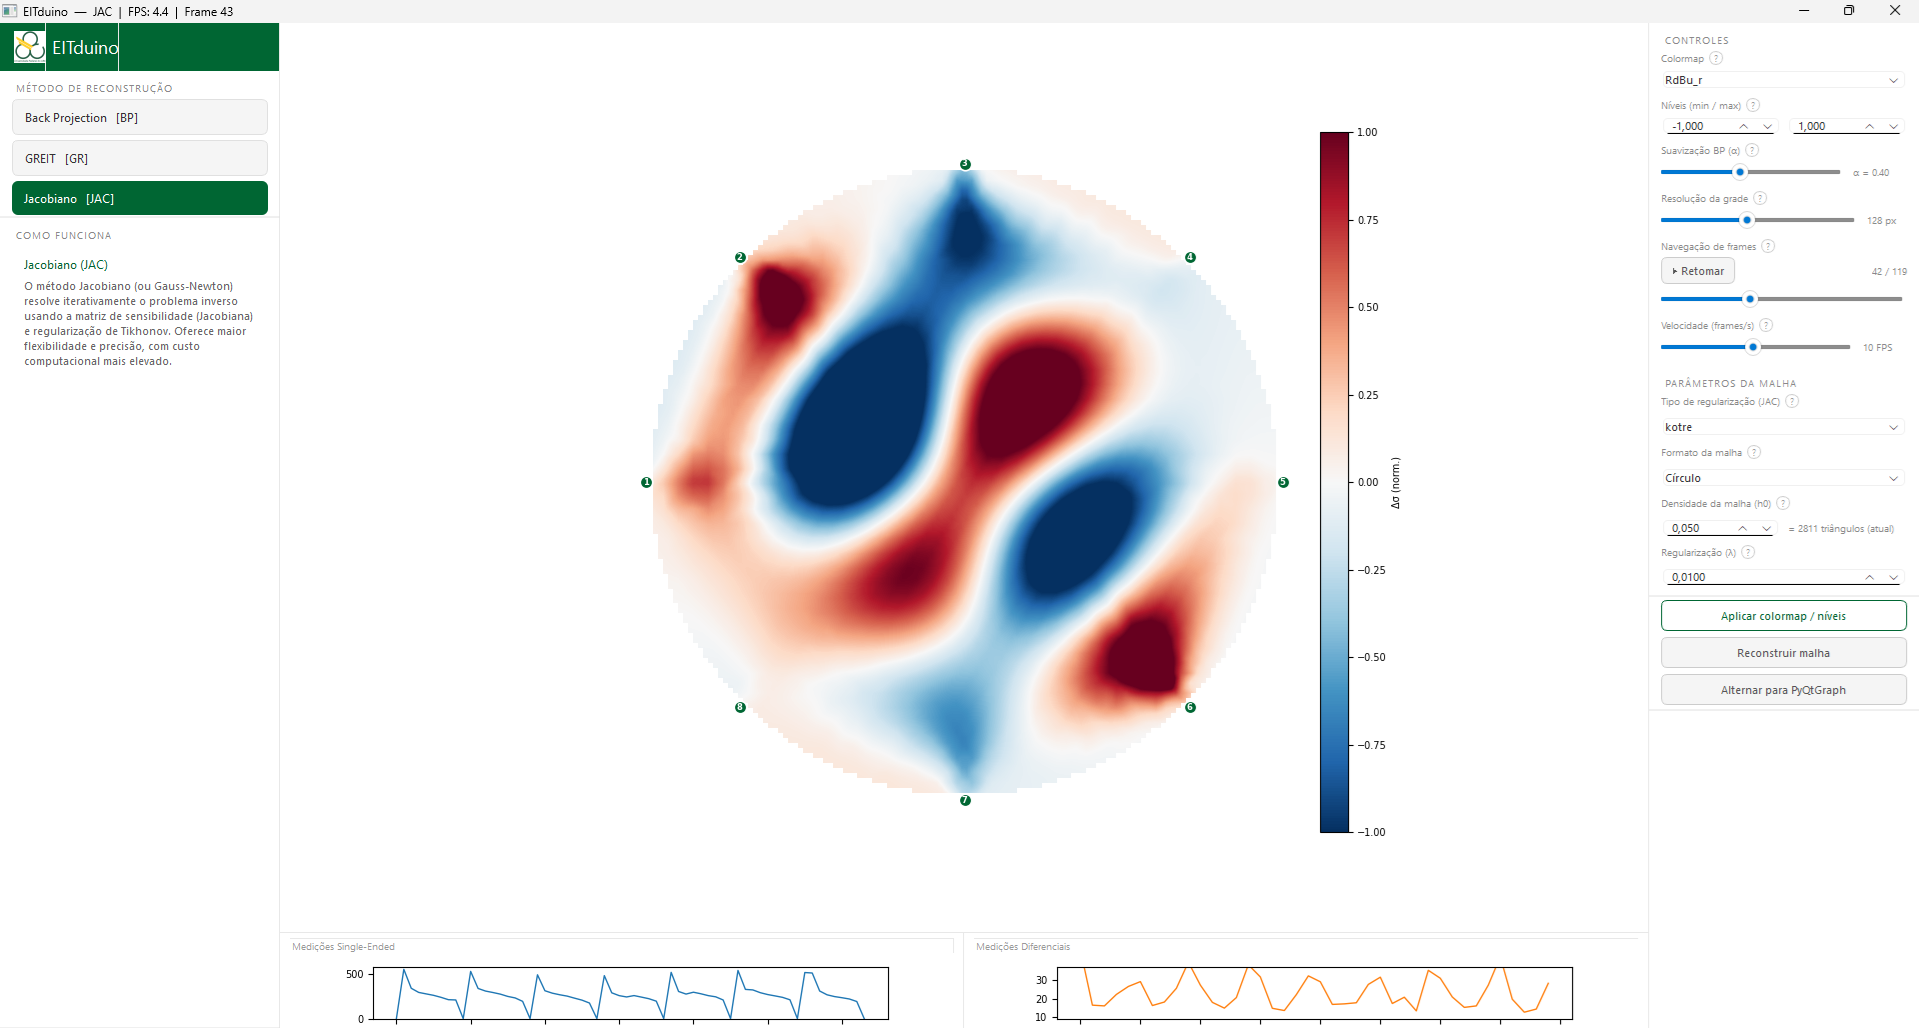
\includegraphics[width=0.85\textwidth]{pictures/JAC_Interface_Frame44_H0_05.png}
    \caption{Visão geral da interface principal com o método Back-Projection ativo (\textit{frame} 43, h0 = 0,10, α = 0,40).}
    \label{fig:interface_geral_bp}
\end{figure}

\section{Comparação entre métodos de reconstrução}
\label{sec:comparacao_metodos}

As figuras a seguir apresentam reconstruções obtidas com os métodos BP, JAC e GREIT em \textit{frame}s consecutivos do mesmo conjunto de dados experimentais. A comparação foi realizada a partir da mesma sequência de medições, mantendo os demais parâmetros de visualização constantes dentro de cada método, de modo a evidenciar diferenças relacionadas ao próprio algoritmo de reconstrução.

No método Back-Projection, mostrado na Figura~\ref{fig:bp_comparacao}, a região associada à haste pode ser identificada na porção superior-central do domínio, sobretudo pela presença de uma área azul mais intensa. Ainda assim, os contornos aparecem difusos e pouco definidos, o que dificulta a delimitação espacial mais precisa do objeto. Também se observam regiões avermelhadas na metade inferior da imagem sem correspondência física evidente com o arranjo experimental, caracterizando artefatos do processo de reconstrução. Entre os \textit{frame}s 43 e 44, a posição geral da região dominante se mantém, mas a imagem permanece espalhada e com baixo contraste local.

No método Jacobiano, apresentado nas Figuras~\ref{fig:jac_frame43} e \ref{fig:jac_frame44}, a posição da haste também é reconstruída na região superior-central do domínio, em concordância com o BP, mas com maior definição espacial e contraste mais localizado. No \textit{frame} 43, observa-se um padrão bipolar de alta intensidade, com alternância marcada entre regiões azuis e vermelhas. No \textit{frame} 44, a reconstrução assume uma forma visualmente mais limpa, com predomínio de uma região azul mais bem definida na área associada ao objeto. A comparação entre os dois \textit{frame}s mostra que o método foi capaz de preservar a localização da haste, mas também exibiu maior sensibilidade às variações entre \textit{frames} consecutivos, resultando em mudanças mais bruscas no padrão visual da reconstrução.

O método GREIT, ilustrado nas Figuras~\ref{fig:greit_frame43} e \ref{fig:greit_frame44}, produziu imagens visualmente mais suaves e estáveis entre \textit{frame}s consecutivos. A região de menor condutividade relativa permanece concentrada na parte superior-central do domínio, em posição compatível com a observada nos demais métodos, o que reforça a consistência qualitativa da localização da haste ao longo da reconstrução. Em contrapartida, o contraste é mais baixo e a transição espacial entre regiões é mais gradual, o que reduz a nitidez dos contornos. Também se destaca a presença de uma borda retangular visível na área reconstruída, decorrente da saída do método em grade regular de pixels. Em conjunto, os três algoritmos localizaram o objeto na mesma região do domínio, diferindo principalmente na definição dos contornos, no contraste e na estabilidade visual entre \textit{frame}s consecutivos.

\begin{figure}[H]
    \centering
    \begin{subfigure}[b]{0.48\textwidth}
        \centering
        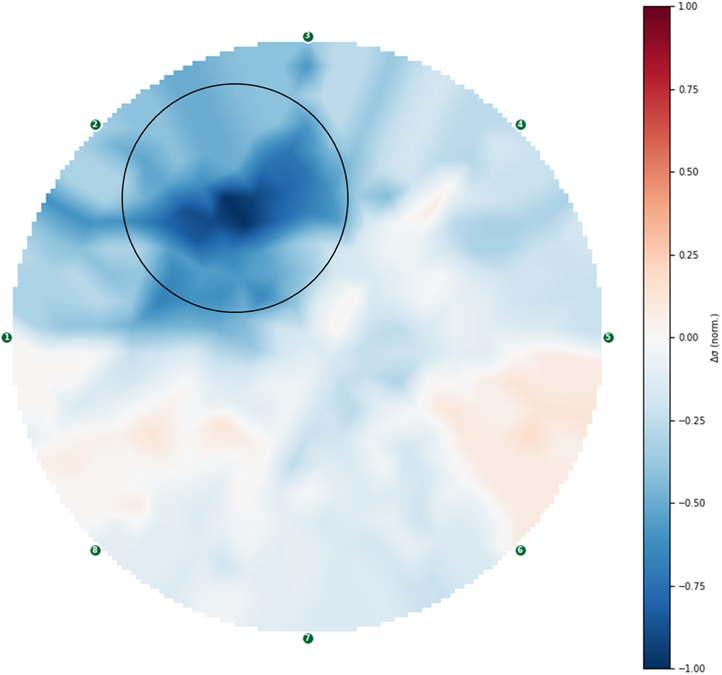
\includegraphics[width=\textwidth]{pictures/BP_Interface_Frame43.png}
        \caption{\textit{Frame} 43}
        \label{fig:bp_frame43}
    \end{subfigure}
    \hfill
    \begin{subfigure}[b]{0.48\textwidth}
        \centering
        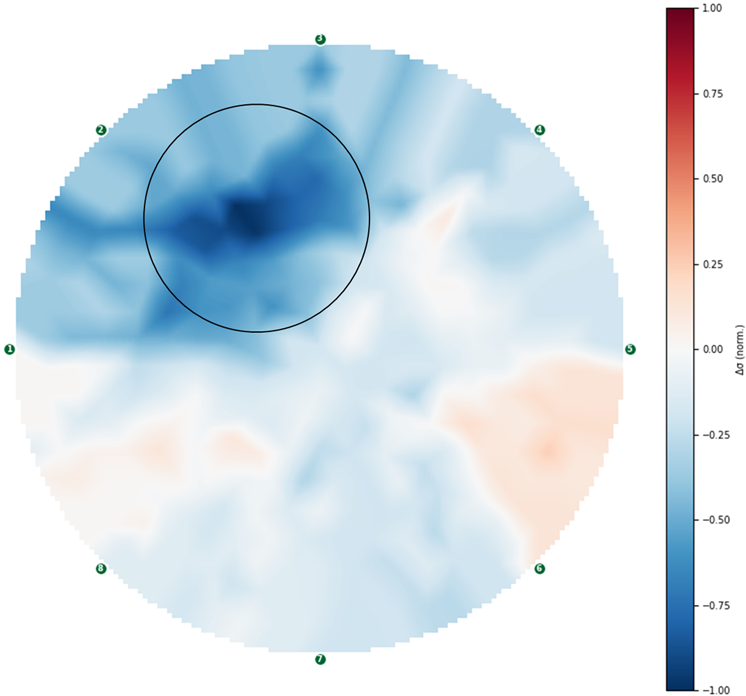
\includegraphics[width=\textwidth]{pictures/BP_Interface_Frame44.png}
        \caption{\textit{Frame} 44}
        \label{fig:bp_frame44}
    \end{subfigure}
    \caption{Reconstruções obtidas com o método Back-Projection (BP). Parâmetros: $h_0 = 0{,}10$, $\alpha = 0{,}40$, colormap \texttt{RdBu\_r}. O círculo indica a região de maior perturbação inferida, compatível com a presença do objeto.}
    \label{fig:bp_comparacao}
\end{figure}

\begin{figure}[H]
    \centering
    \begin{subfigure}[b]{0.48\textwidth}
        \centering
        
\includegraphics[width=\textwidth]{pictures/JAC_Interface_Frame43.png}
        \caption{\textit{Frame} 43}
        \label{fig:jac_frame43}
    \end{subfigure}
    \hfill
    \begin{subfigure}[b]{0.48\textwidth}
        \centering
        
\includegraphics[width=\textwidth]{pictures/JAC_Interface_Frame44.png}
        \caption{\textit{Frame} 44}
        \label{fig:jac_frame44}
    \end{subfigure}
    \caption{Reconstruções obtidas com o método Jacobiano (JAC). Parâmetros: \(h_0 = 0{,}10\), regularização \(\lambda = 0{,}0100\), método \texttt{kotre}, colormap \texttt{RdBu\_r}. O círculo indica a região de maior perturbação de condutividade inferida.}
    \label{fig:jac_comparacao}
\end{figure}

\begin{figure}[H]
    \centering
    \begin{subfigure}[b]{0.48\textwidth}
    \centering
    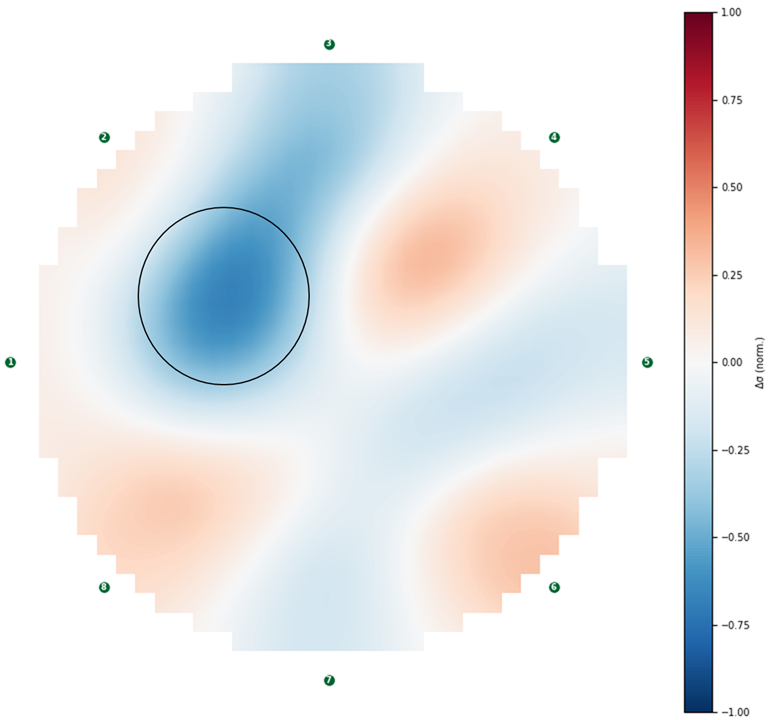
\includegraphics[width=\textwidth]{pictures/GREIT_Interface_Frame43.png}
    \caption{\textit{Frame} 43}
    \label{fig:greit_frame43}
    \end{subfigure}
    \hfill
    \begin{subfigure}[b]{0.48\textwidth}
        \centering
        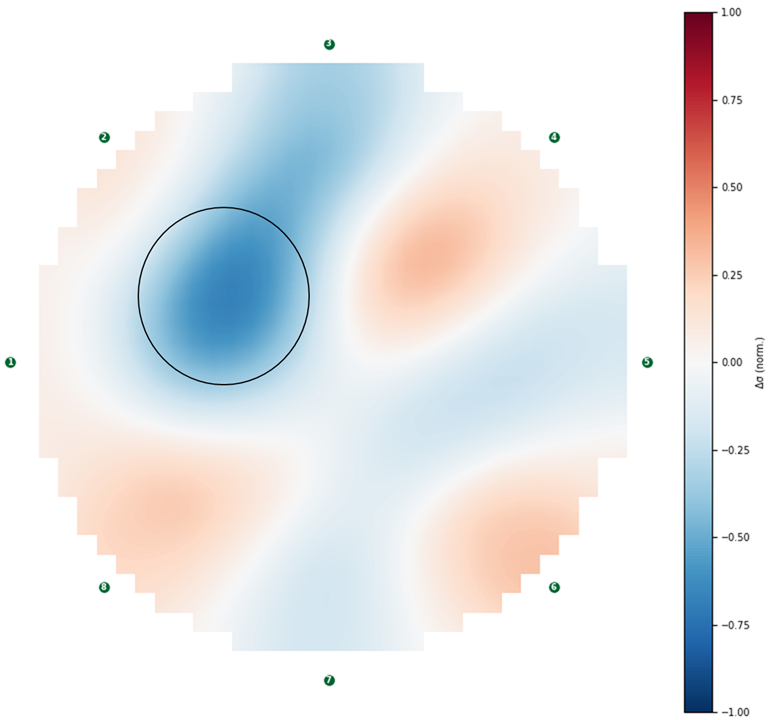
\includegraphics[width=\textwidth]{pictures/GREIT_Interface_Frame44.png}
        \caption{\textit{Frame} 44}
        \label{fig:greit_frame44}
    \end{subfigure}
    \caption{Reconstruções obtidas com o método GREIT. Parâmetros: \(h_0 = 0{,}10\), resolução da grade \(= 128\), colormap \texttt{RdBu\_r}. O círculo indica a região de maior perturbação de condutividade inferida.}
    \label{fig:greit_comparacao}
\end{figure}

\section{Efeito dos parâmetros configuráveis}
\label{sec:efeito_parametros}

\subsection{Densidade da malha (\(h_0\))}
\label{subsec:efeito_h0}

O parâmetro \(h_0\) define o comprimento máximo de aresta dos elementos triangulares da malha, expresso em unidades normalizadas em relação ao raio do domínio. Valores menores de \(h_0\) resultam em malhas mais refinadas, com maior número de elementos e resolução espacial mais alta, ao custo de maior custo computacional por quadro reconstruído.

As Figuras~\ref{fig:jac_h005} e \ref{fig:jac_h020} mostram o efeito da variação do parâmetro \(h_0\) na reconstrução obtida com o método Jacobiano. Na configuração mais refinada, com \(h_0 = 0{,}05\), a interface indica uma malha com 2811 triângulos, resultando em uma reconstrução visualmente mais detalhada, porém também mais fragmentada e com maior presença de artefatos locais. Na configuração mais grossa, com \(h_0 = 0{,}20\), a malha passa a conter 160 triângulos, produzindo uma imagem mais simples e suave, com menor nível de fragmentação. Essa comparação mostra que o refinamento da malha amplia a complexidade espacial da reconstrução, ao custo de maior carga computacional por quadro, dado o maior número de elementos envolvidos no cálculo.

\begin{figure}[htbp]
    \centering
    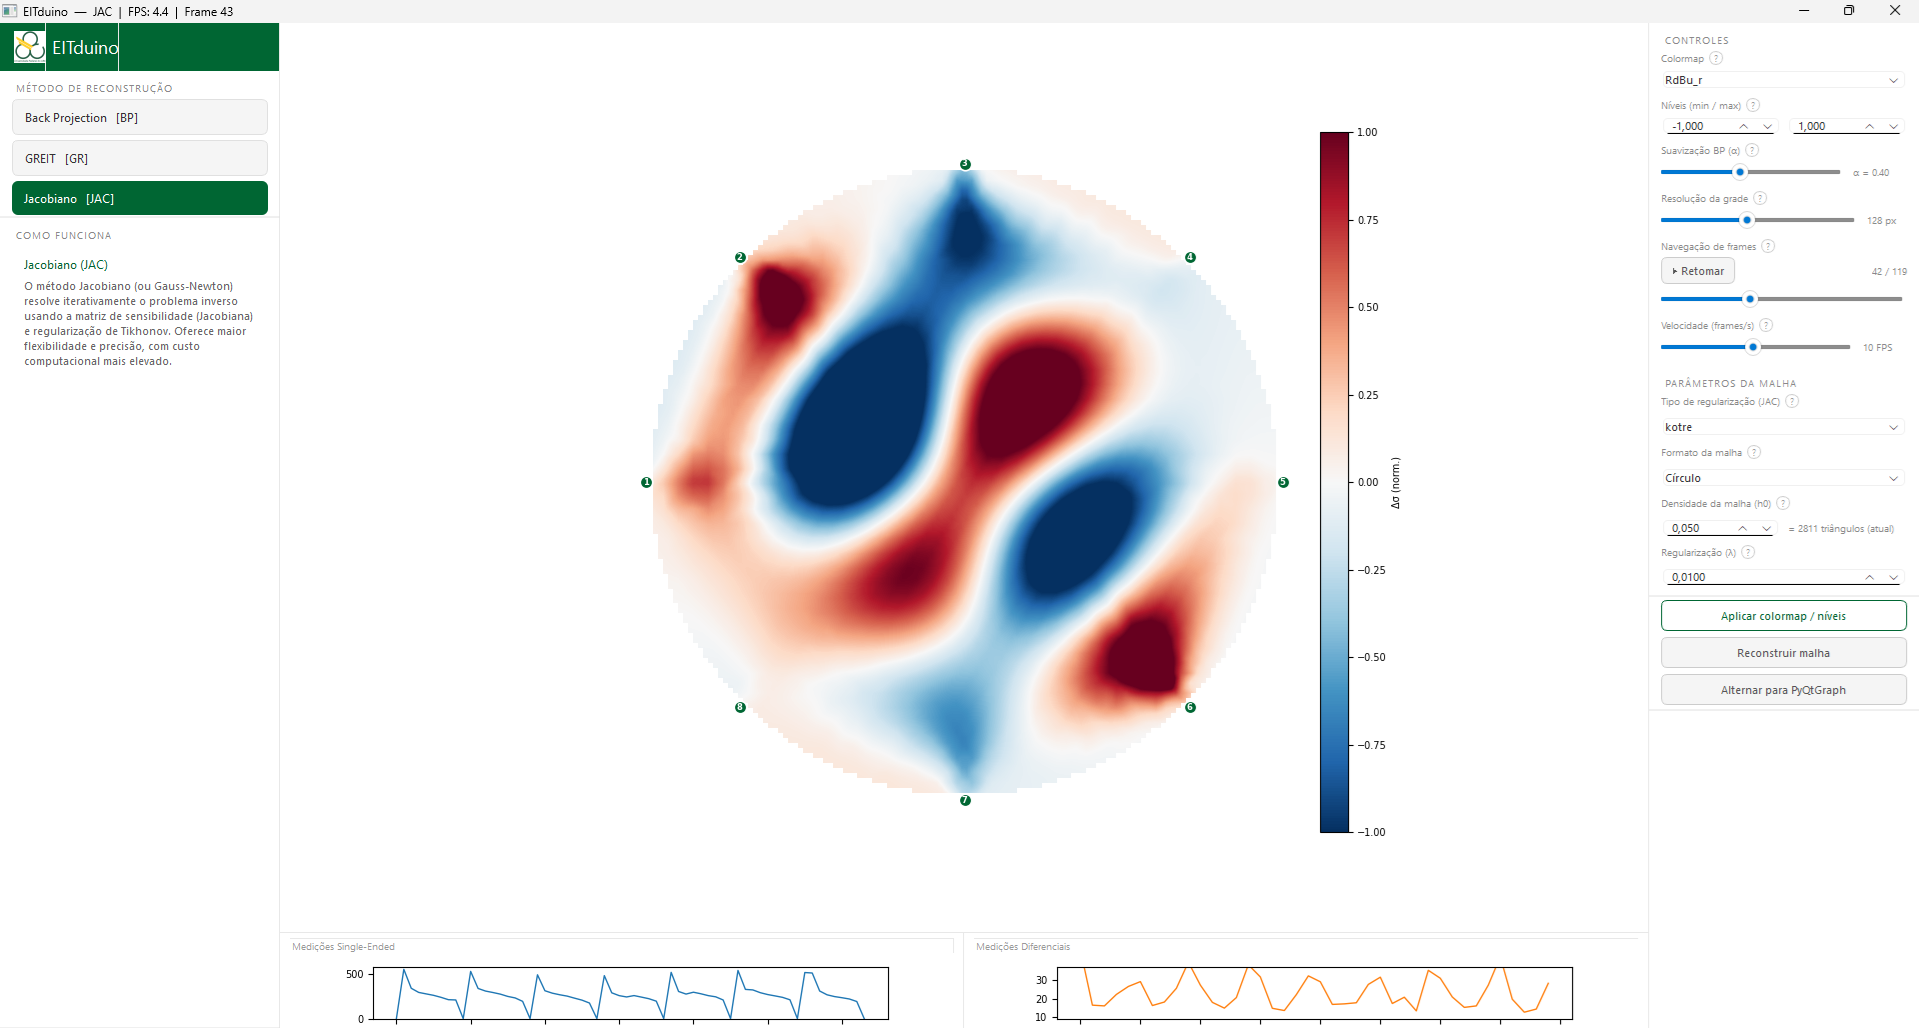
\includegraphics[width=0.85\textwidth]{pictures/JAC_Interface_Frame44_H0_05.png}
    \caption{Reconstrução obtida com o método Jacobiano no \textit{frame} 44, utilizando \(h_0 = 0{,}05\). A interface indica uma malha com 2811 triângulos.}
    \label{fig:jac_h005}
\end{figure}

\begin{figure}[htbp]
    \centering
    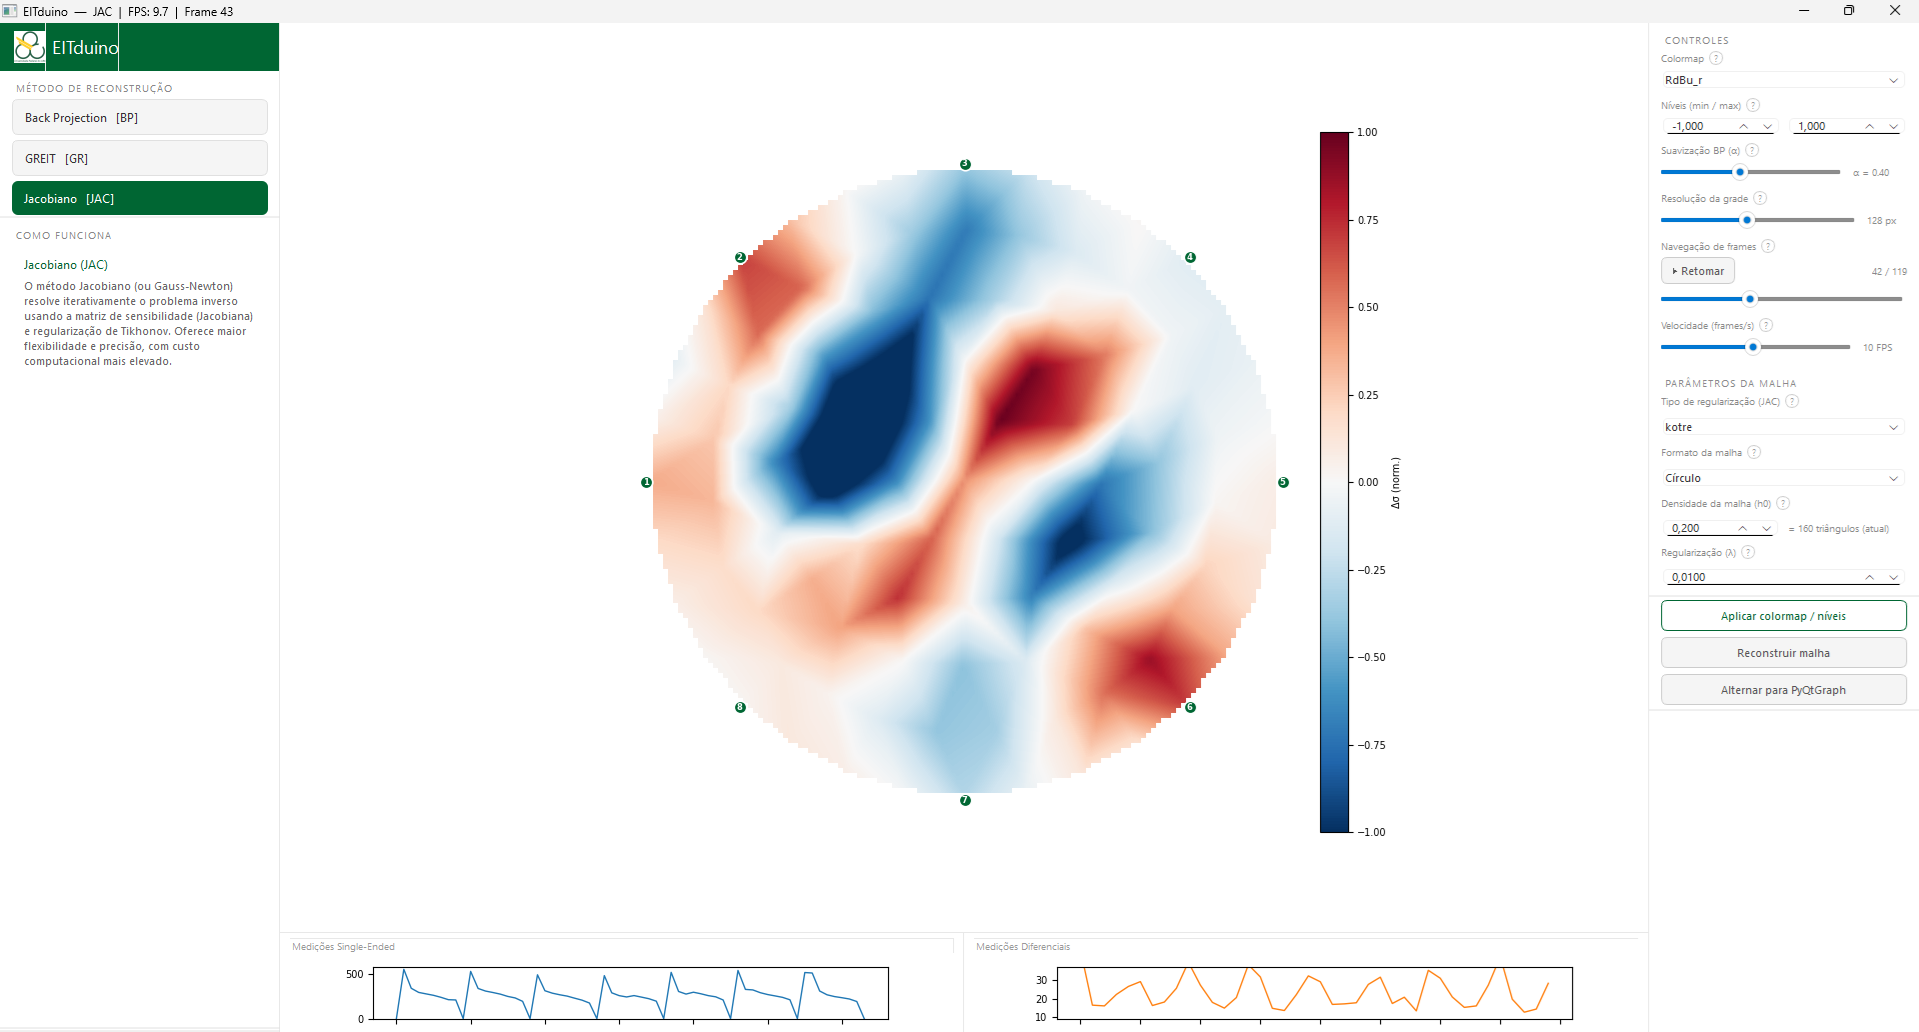
\includegraphics[width=0.85\textwidth]{pictures/JAC_Interface_Frame44_H0_2.png}
    \caption{Reconstrução obtida com o método Jacobiano no \textit{frame} 44, utilizando \(h_0 = 0{,}20\). A interface indica uma malha com 160 triângulos.}
    \label{fig:jac_h020}
\end{figure}

\subsection{Suavização temporal (\(\alpha\))}
\label{subsec:efeito_alpha}

O parâmetro \(\alpha \in [0, 1]\) é adimensional e controla o peso atribuído à reconstrução do quadro anterior na composição da imagem exibida, conforme definido na Equação~\ref{eq:suavizacao_temporal}.

As Figuras~\ref{fig:bp_alpha01} e \ref{fig:bp_alpha09} ilustram o efeito do parâmetro de suavização temporal \(\alpha\) nas reconstruções obtidas com o método Back-Projection. Com \(\alpha = 0{,}10\), a imagem responde mais diretamente ao \textit{frame} corrente, preservando com maior fidelidade as variações instantâneas, mas também exibindo maior oscilação visual. Com \(\alpha = 0{,}90\), a reconstrução passa a variar de forma mais gradual entre \textit{frames}, produzindo um resultado visualmente mais estável. A comparação entre essas duas configurações mostra que o aumento de \(\alpha\) reduz a cintilação entre \textit{frames} consecutivos, embora também introduza um leve fator de inércia na resposta visual do método. Como o efeito da suavização temporal se manifesta principalmente na transição entre quadros consecutivos, sua influência é mais evidente durante a reprodução animada dos dados do que na comparação entre imagens estáticas.

\begin{figure}[htbp]
    \centering
    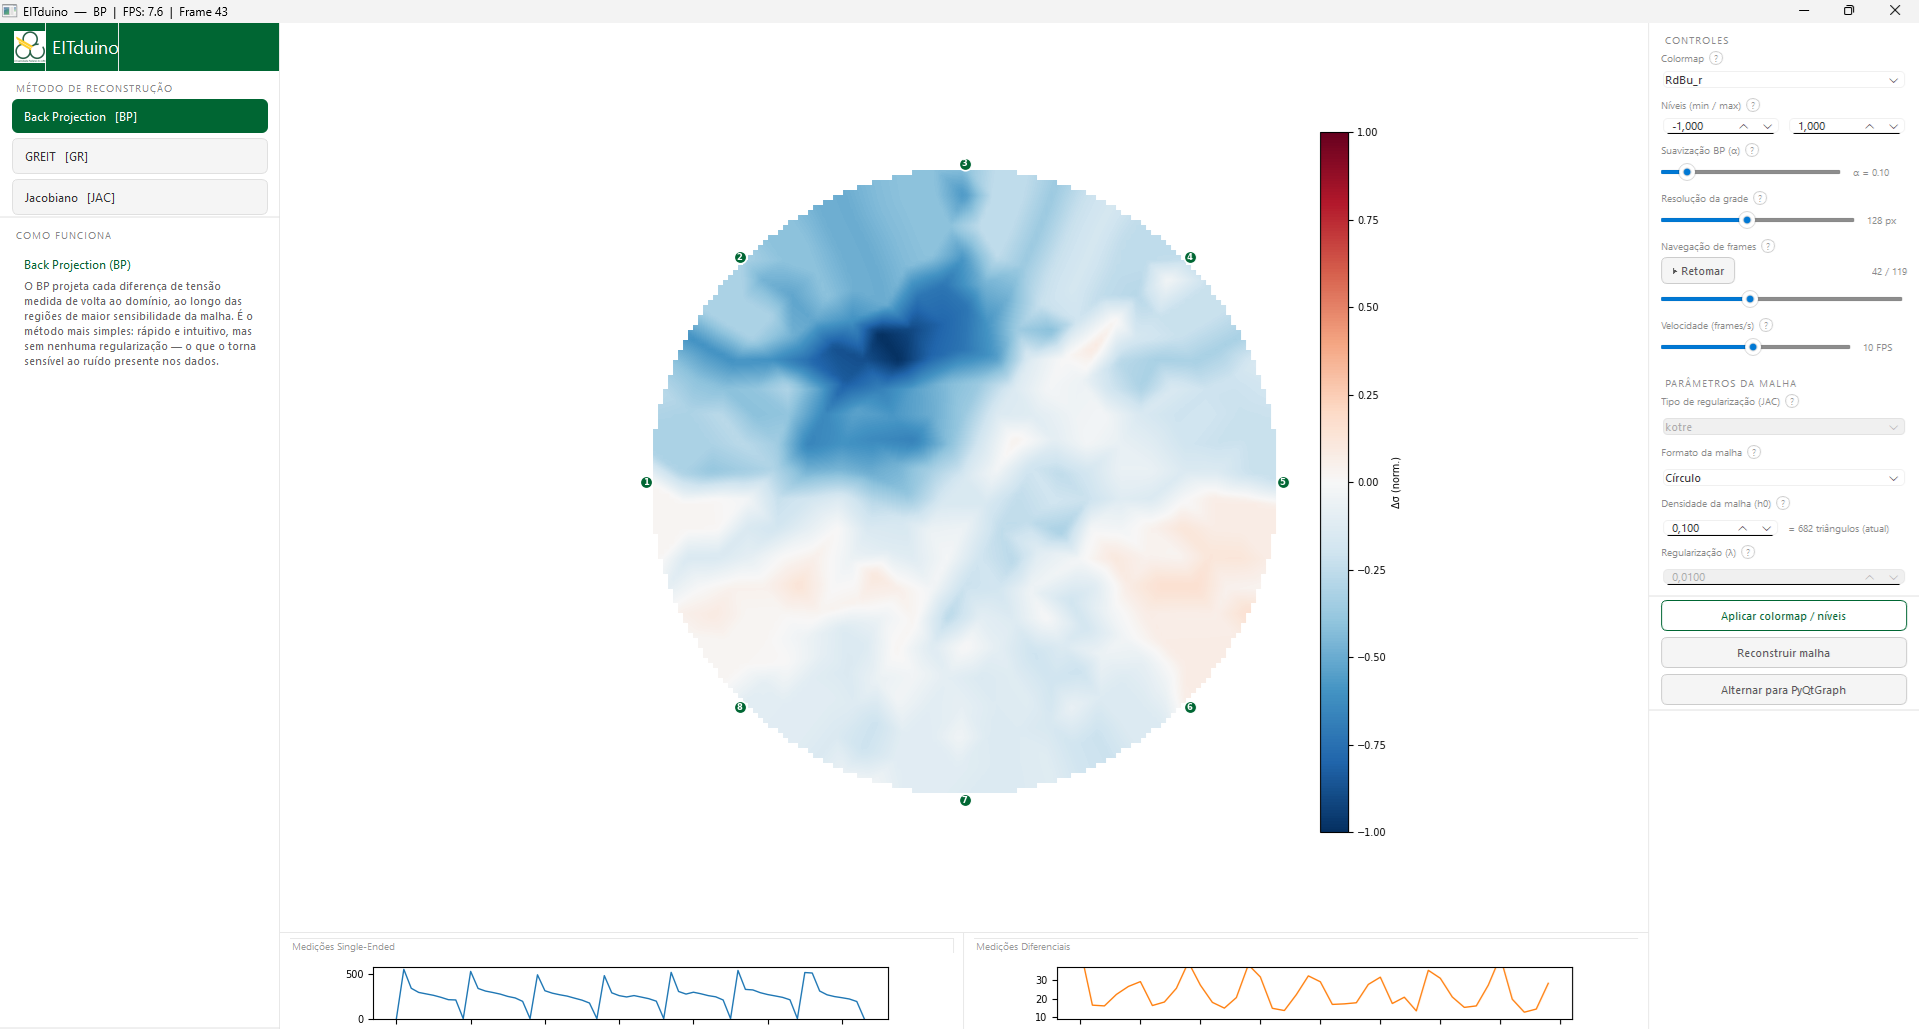
\includegraphics[width=0.85\textwidth]{pictures/BP_Interface_Frame43_alpha0_1.png}
    \caption{Reconstrução obtida com o método Back-Projection no \textit{frame} 43, utilizando \(\alpha = 0{,}10\).}
    \label{fig:bp_alpha01}
\end{figure}

\begin{figure}[htbp]
    \centering
    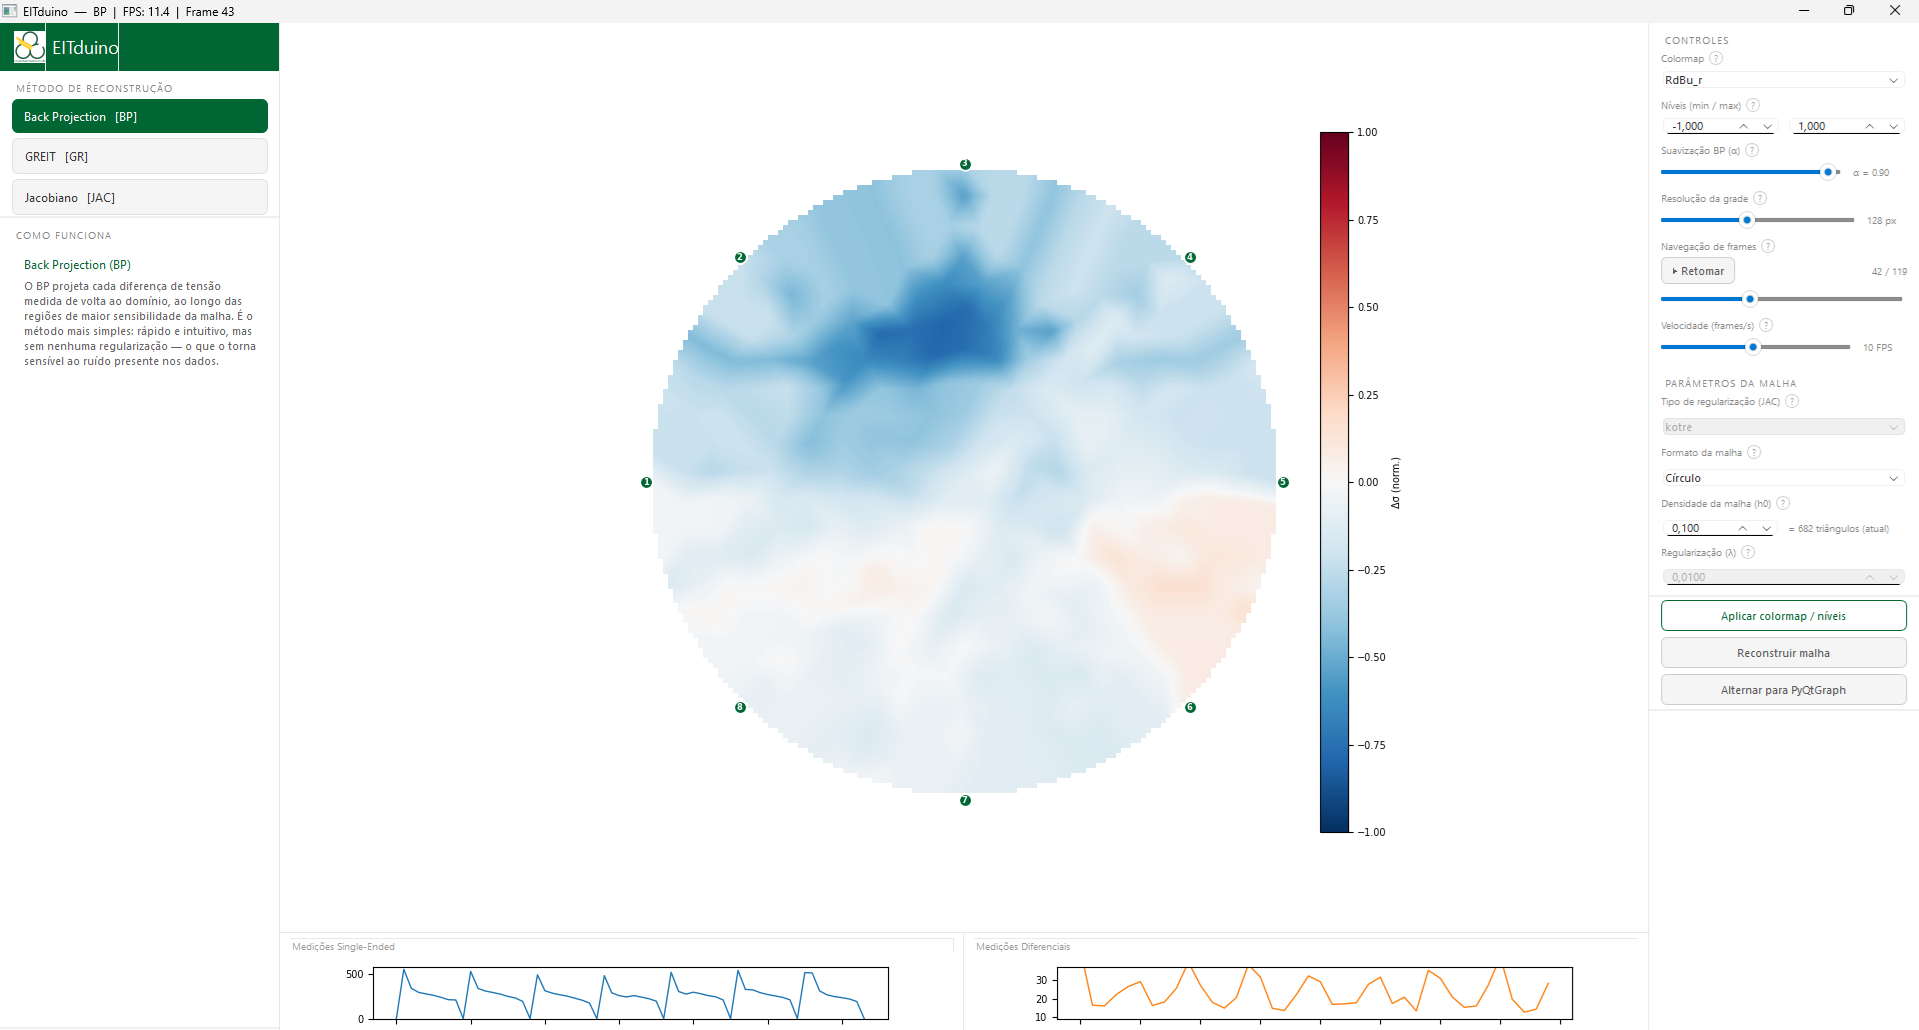
\includegraphics[width=0.85\textwidth]{pictures/BP_Interface_Frame43_alpha0_9.png}
    \caption{Reconstrução obtida com o método Back-Projection no \textit{frame} 43, utilizando \(\alpha = 0{,}90\).}
    \label{fig:bp_alpha09}
\end{figure}

\subsection{Efeito da regularização (\(\lambda\))}
\label{subsec:efeito_regularizacao}

As Figuras~\ref{fig:jac_reg_0001} a \ref{fig:greit_reg_1} mostram o efeito da variação do parâmetro de regularização \(\lambda\) nas reconstruções obtidas com os métodos Jacobiano e GREIT. Para essa comparação, foi utilizado o mesmo \textit{frame} do conjunto experimental, mantendo-se constantes a geometria da malha, o valor de \(h_0\), a resolução da grade e os demais parâmetros de visualização. Foram testados quatro valores de regularização em cada método: \(\lambda = 0{,}0001\), \(\lambda = 0{,}01\), \(\lambda = 0{,}1\) e \(\lambda = 1{,}0\).

No caso do método Jacobiano, a progressão entre as Figuras~\ref{fig:jac_reg_0001}, \ref{fig:jac_reg_001}, \ref{fig:jac_reg_01} e \ref{fig:jac_reg_1} evidencia de forma clara o efeito da regularização sobre a reconstrução. Com \(\lambda = 0{,}0001\), a imagem apresenta alto contraste, contornos mais agudos e forte presença de artefatos bipolares, indicando predominância da aderência aos dados medidos sobre a suavização da solução. Com \(\lambda = 0{,}01\), o padrão visual permanece semelhante, mas ligeiramente mais contido. Em \(\lambda = 0{,}1\), a reconstrução torna-se visivelmente mais suave, com redução dos artefatos mais intensos e uma localização mais legível da região associada à haste. Já com \(\lambda = 1{,}0\), a imagem fica amplamente atenuada, restando apenas uma região azul difusa e de baixo contraste, o que indica predominância da regularização sobre a contribuição dos dados experimentais.

No método GREIT, observa-se comportamento análogo, embora com o padrão espacial característico do próprio algoritmo. Nas Figuras~\ref{fig:greit_reg_0001} e \ref{fig:greit_reg_001}, a reconstrução exibe regiões azul-vermelho bem definidas e com maior contraste, ainda com forte influência do termo de dados. Na Figura~\ref{fig:greit_reg_01}, o padrão torna-se mais suave e menos intenso, com transições espaciais mais graduais. Na Figura~\ref{fig:greit_reg_1}, a imagem aparece quase completamente suprimida, permanecendo apenas uma variação residual de baixa intensidade. Em ambos os métodos, a transição entre imagens mais nítidas e mais ruidosas para imagens mais suaves e mais atenuadas torna visível, na própria interface, o compromisso entre fidelidade aos dados e estabilidade da solução.

Esse comportamento está de acordo com a formulação teórica apresentada para o problema inverso regularizado: a escolha de \(\lambda\) controla diretamente o equilíbrio entre aderência às medições e suavização da reconstrução, efeito que pode ser observado qualitativamente de forma imediata na interface desenvolvida.

\begin{figure}[htbp]
    \centering
    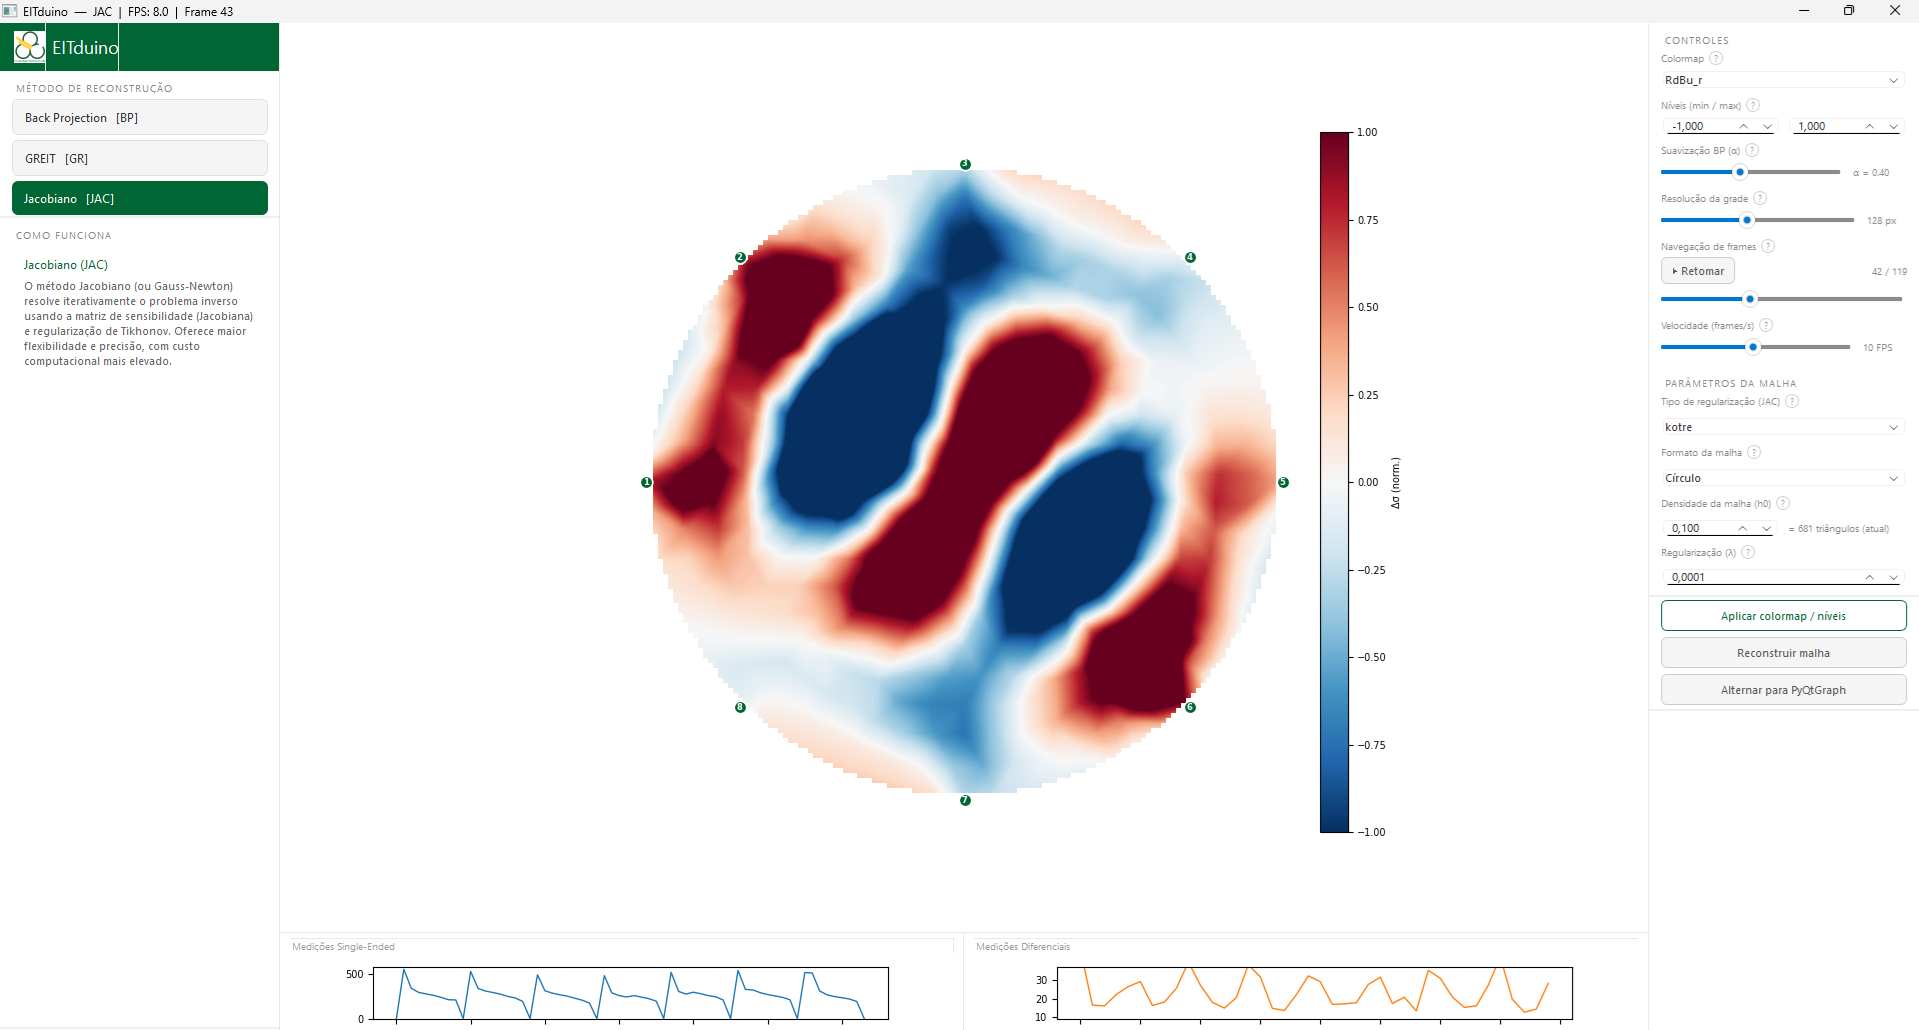
\includegraphics[width=0.85\textwidth]{pictures/JAC_pyQT_Reg0_0001.png}
    \caption{Reconstrução obtida com o método Jacobiano no \textit{frame} 43, utilizando \(\lambda = 0{,}0001\).}
    \label{fig:jac_reg_0001}
\end{figure}

\begin{figure}[htbp]
    \centering
    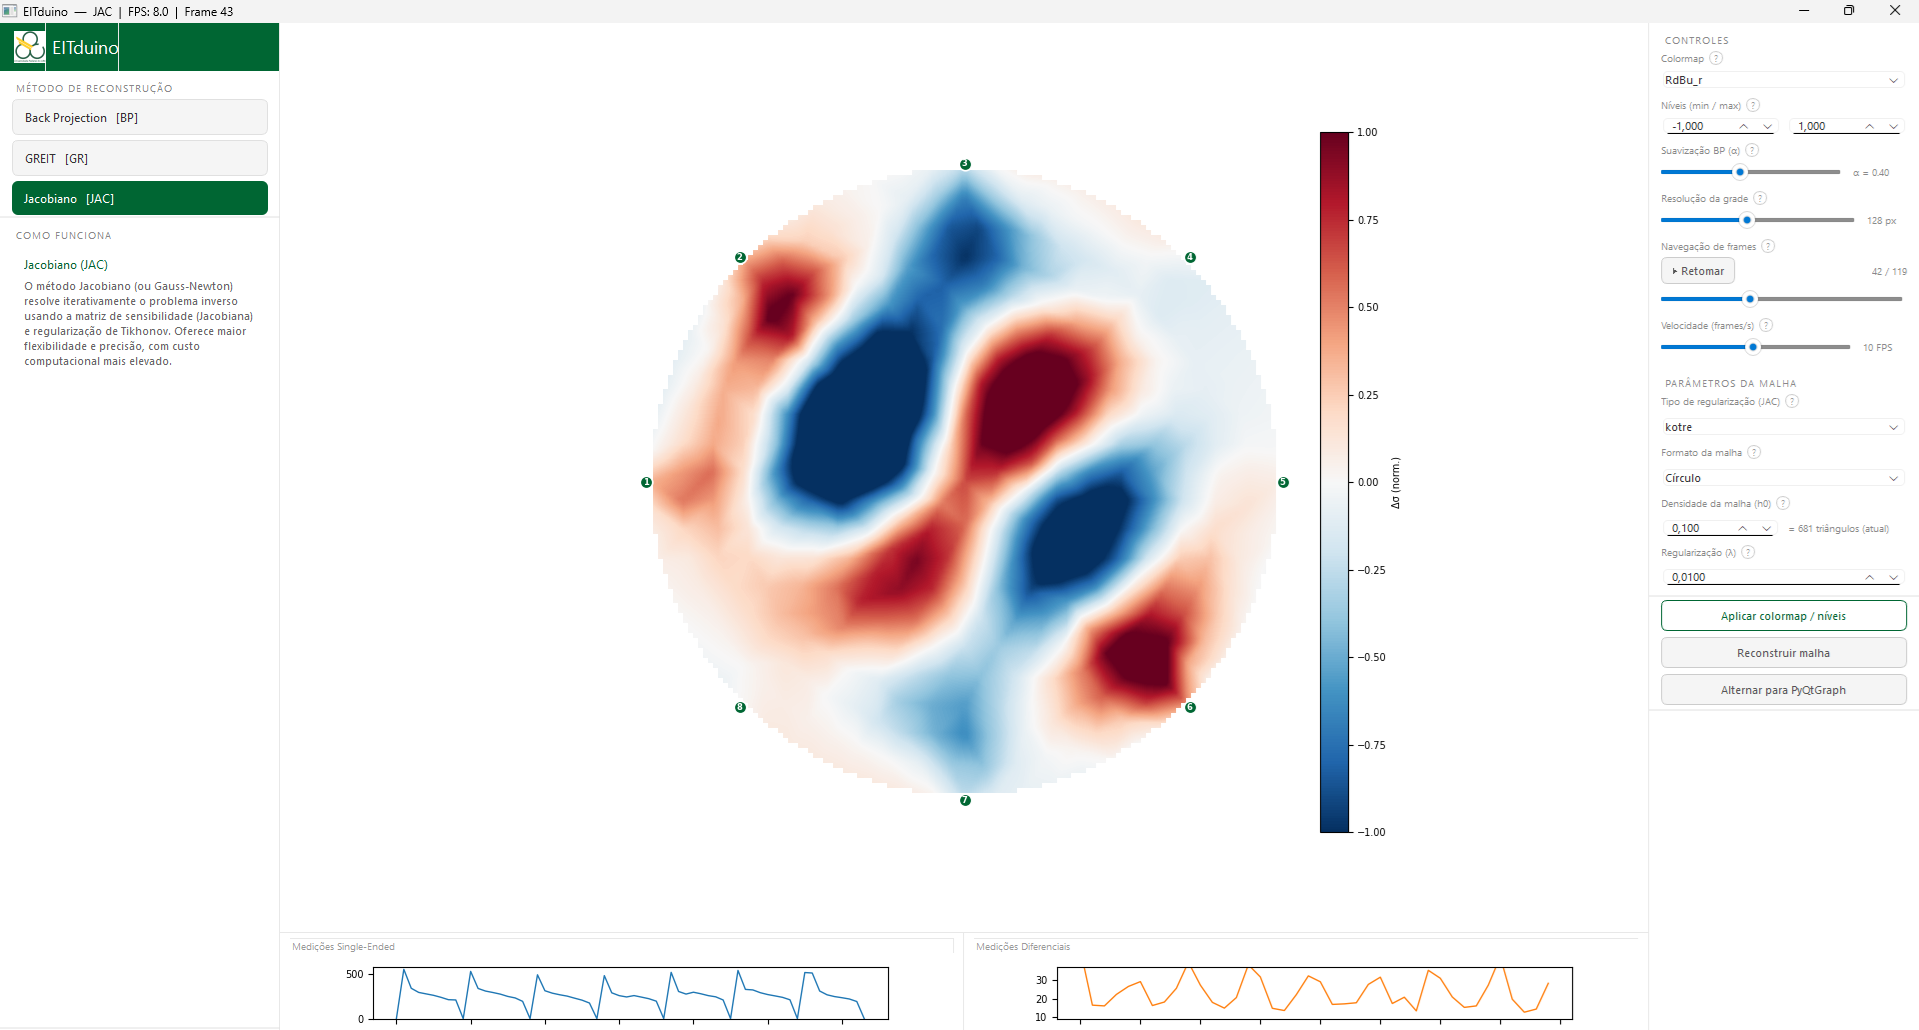
\includegraphics[width=0.85\textwidth]{pictures/JAC_pyQT_Reg0_01.png}
    \caption{Reconstrução obtida com o método Jacobiano no \textit{frame} 43, utilizando \(\lambda = 0{,}01\).}
    \label{fig:jac_reg_001}
\end{figure}

\begin{figure}[htbp]
    \centering
    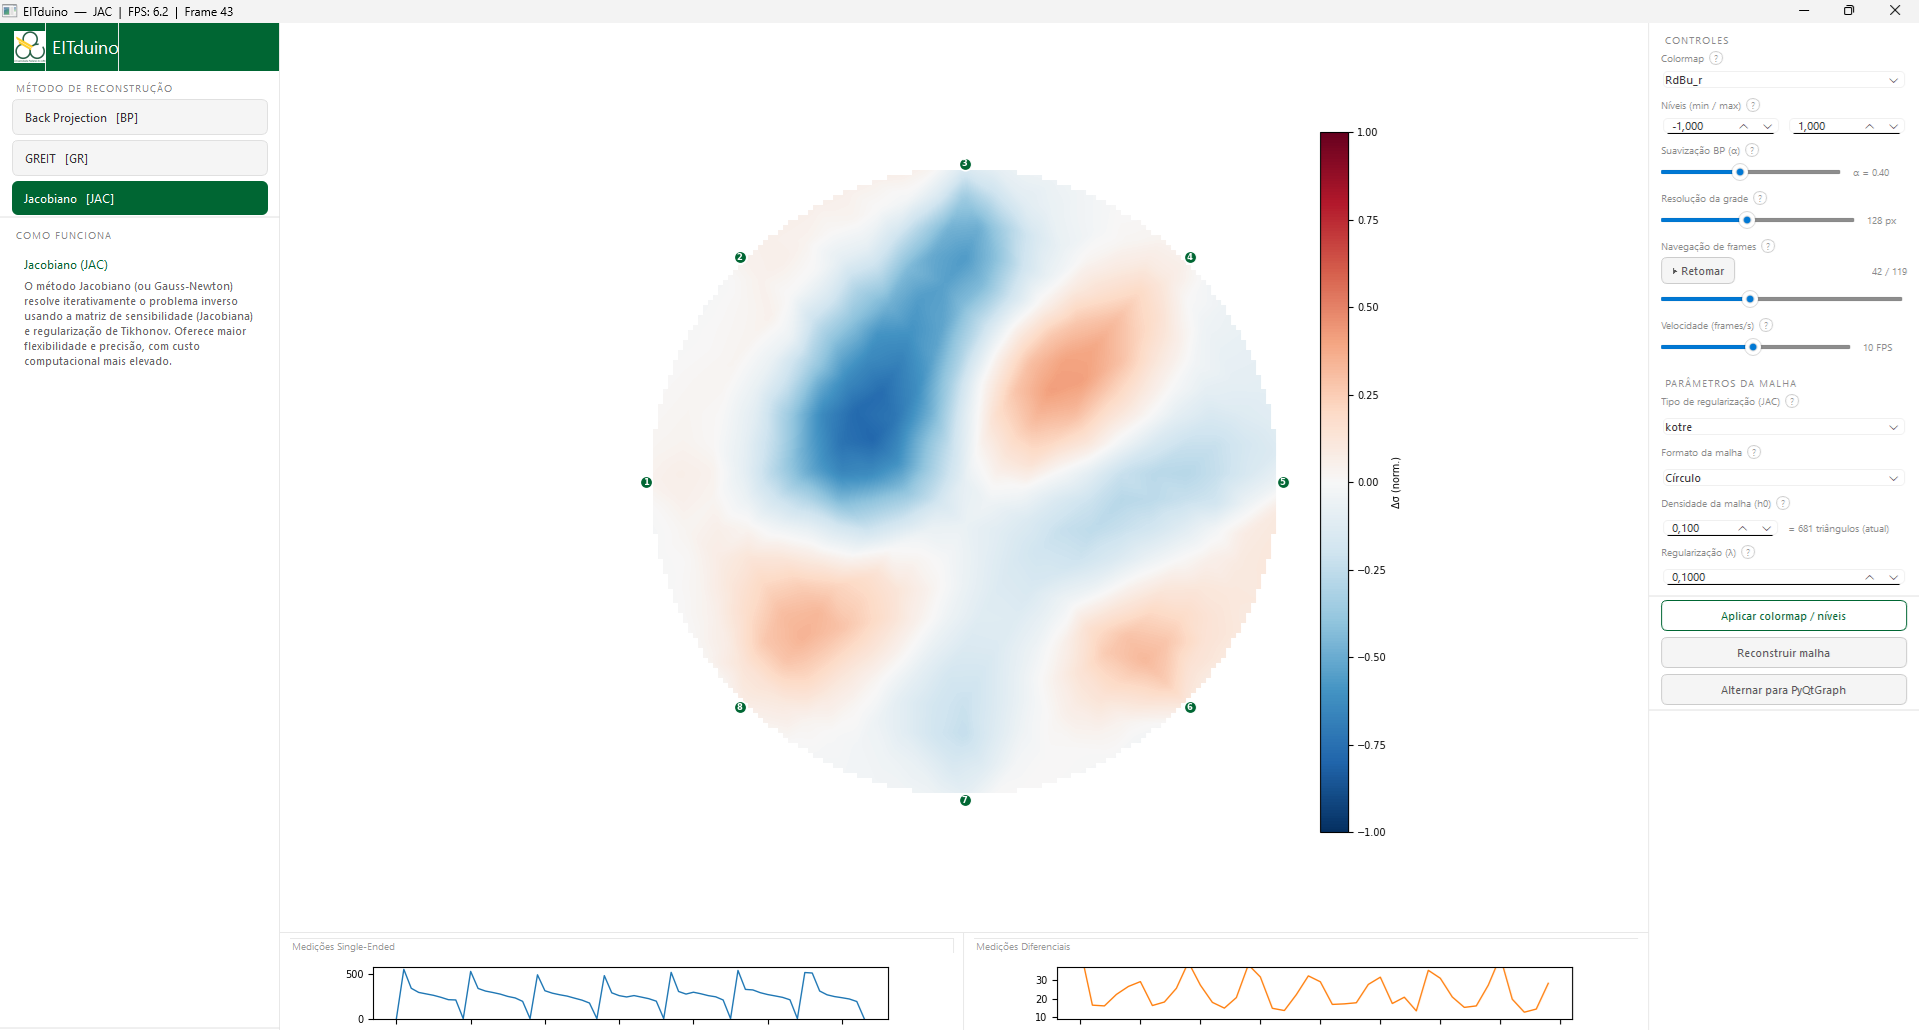
\includegraphics[width=0.85\textwidth]{pictures/JAC_pyQT_Reg0_1.png}
    \caption{Reconstrução obtida com o método Jacobiano no \textit{frame} 43, utilizando \(\lambda = 0{,}1\).}
    \label{fig:jac_reg_01}
\end{figure}

\begin{figure}[htbp]
    \centering
    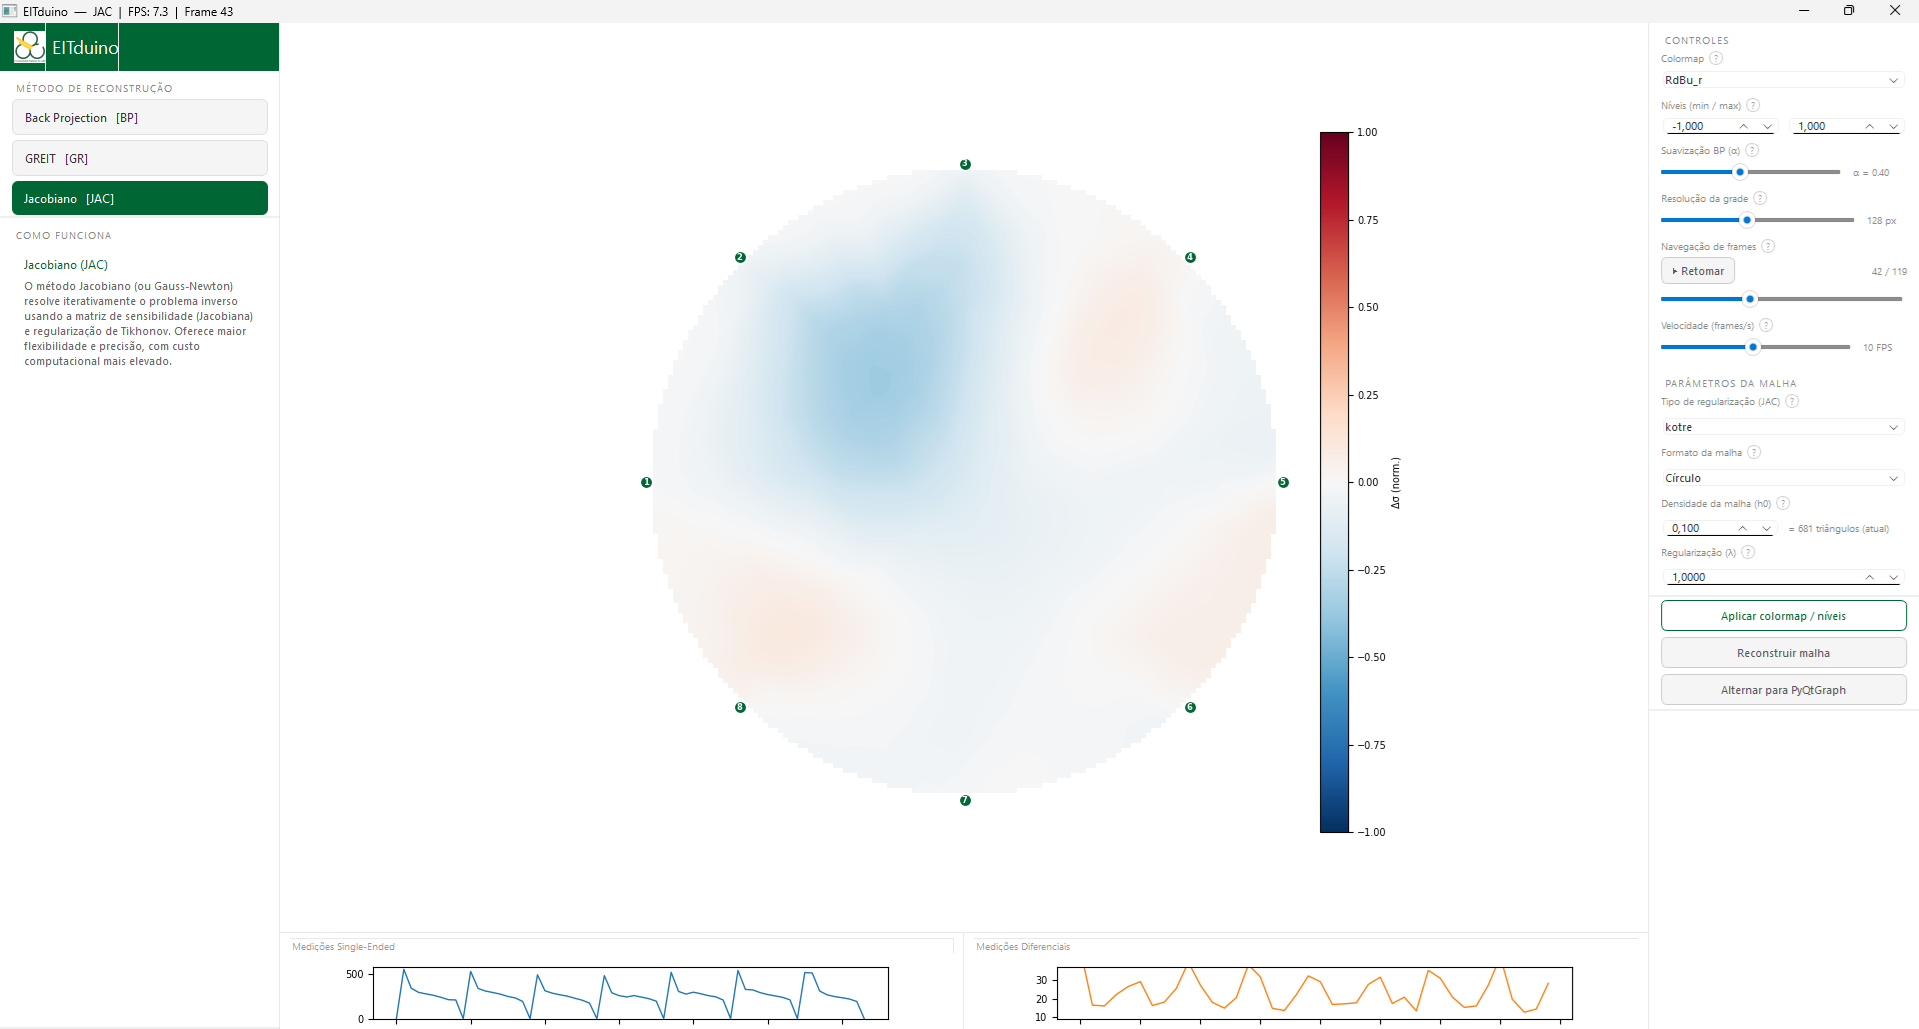
\includegraphics[width=0.85\textwidth]{pictures/JAC_pyQT_Reg1.png}
    \caption{Reconstrução obtida com o método Jacobiano no \textit{frame} 43, utilizando \(\lambda = 1{,}0\).}
    \label{fig:jac_reg_1}
\end{figure}

\begin{figure}[htbp]
    \centering
    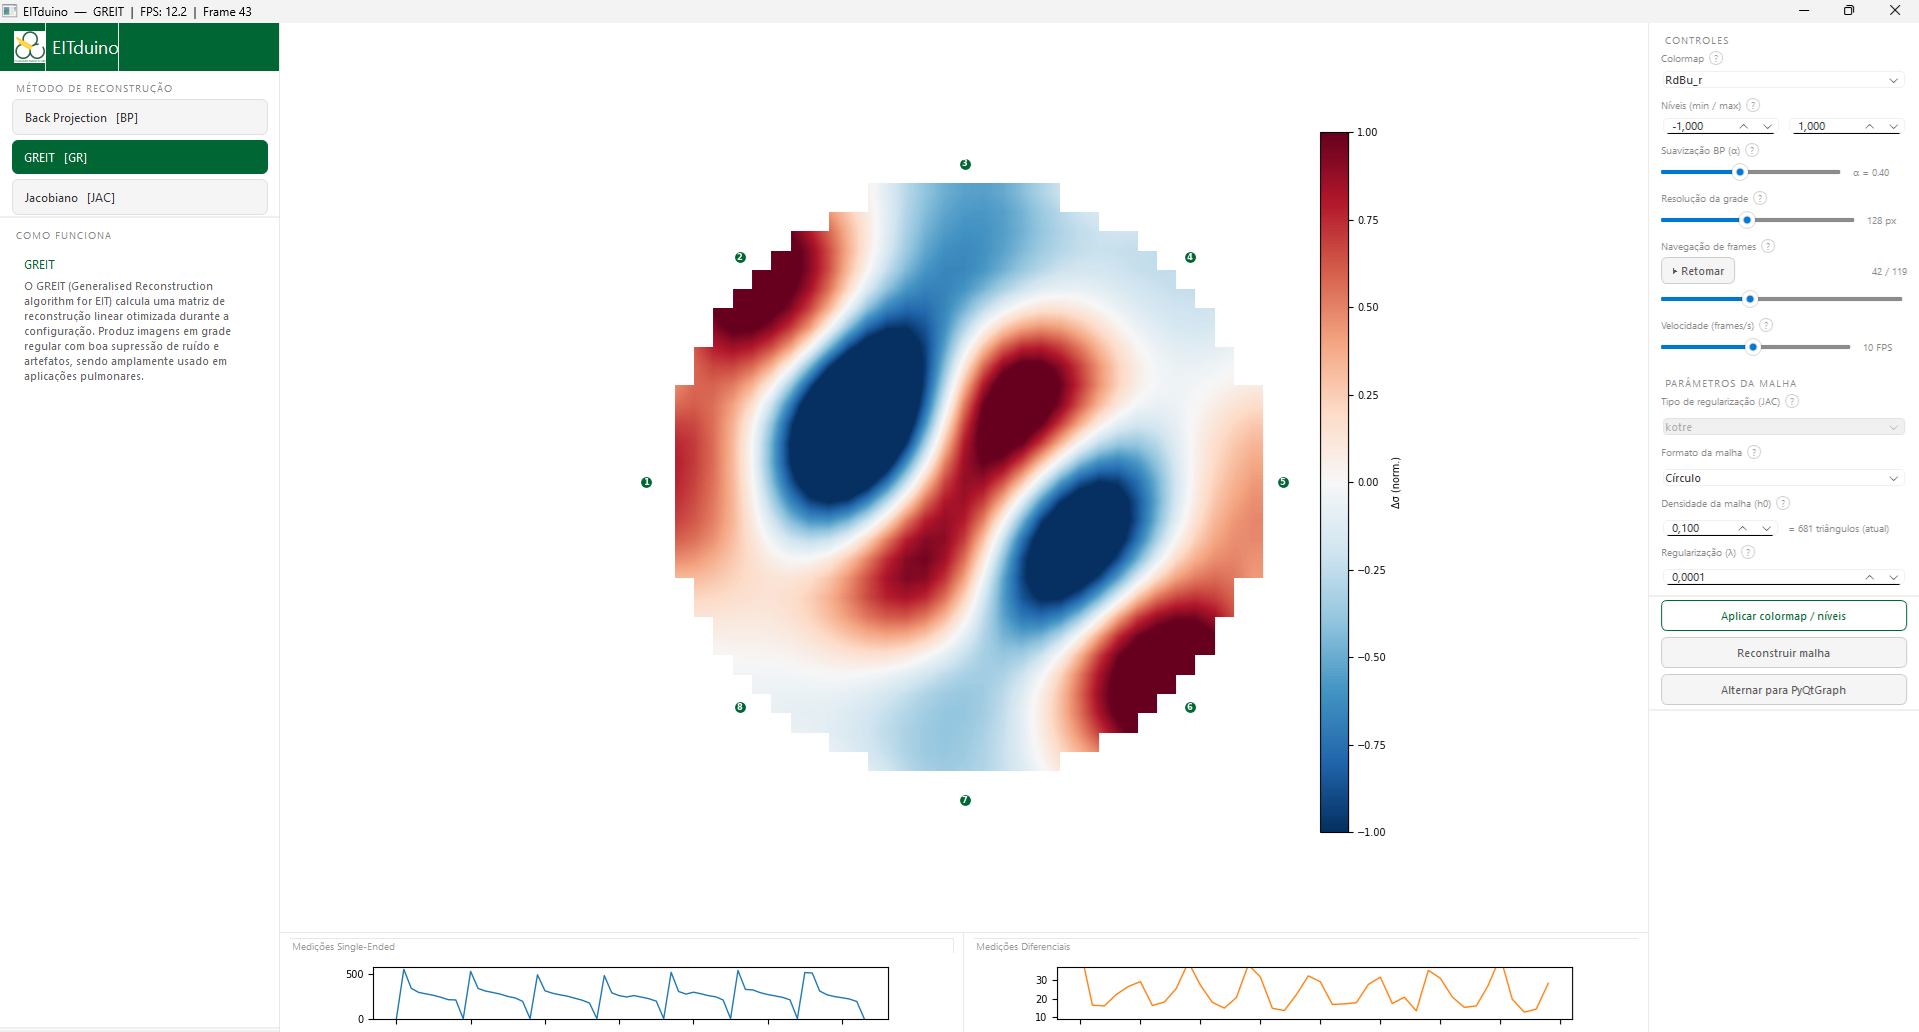
\includegraphics[width=0.85\textwidth]{pictures/GREIT_pyQT_Reg0_0001.png}
    \caption{Reconstrução obtida com o método GREIT no \textit{frame} 43, utilizando \(\lambda = 0{,}0001\).}
    \label{fig:greit_reg_0001}
\end{figure}

\begin{figure}[htbp]
    \centering
    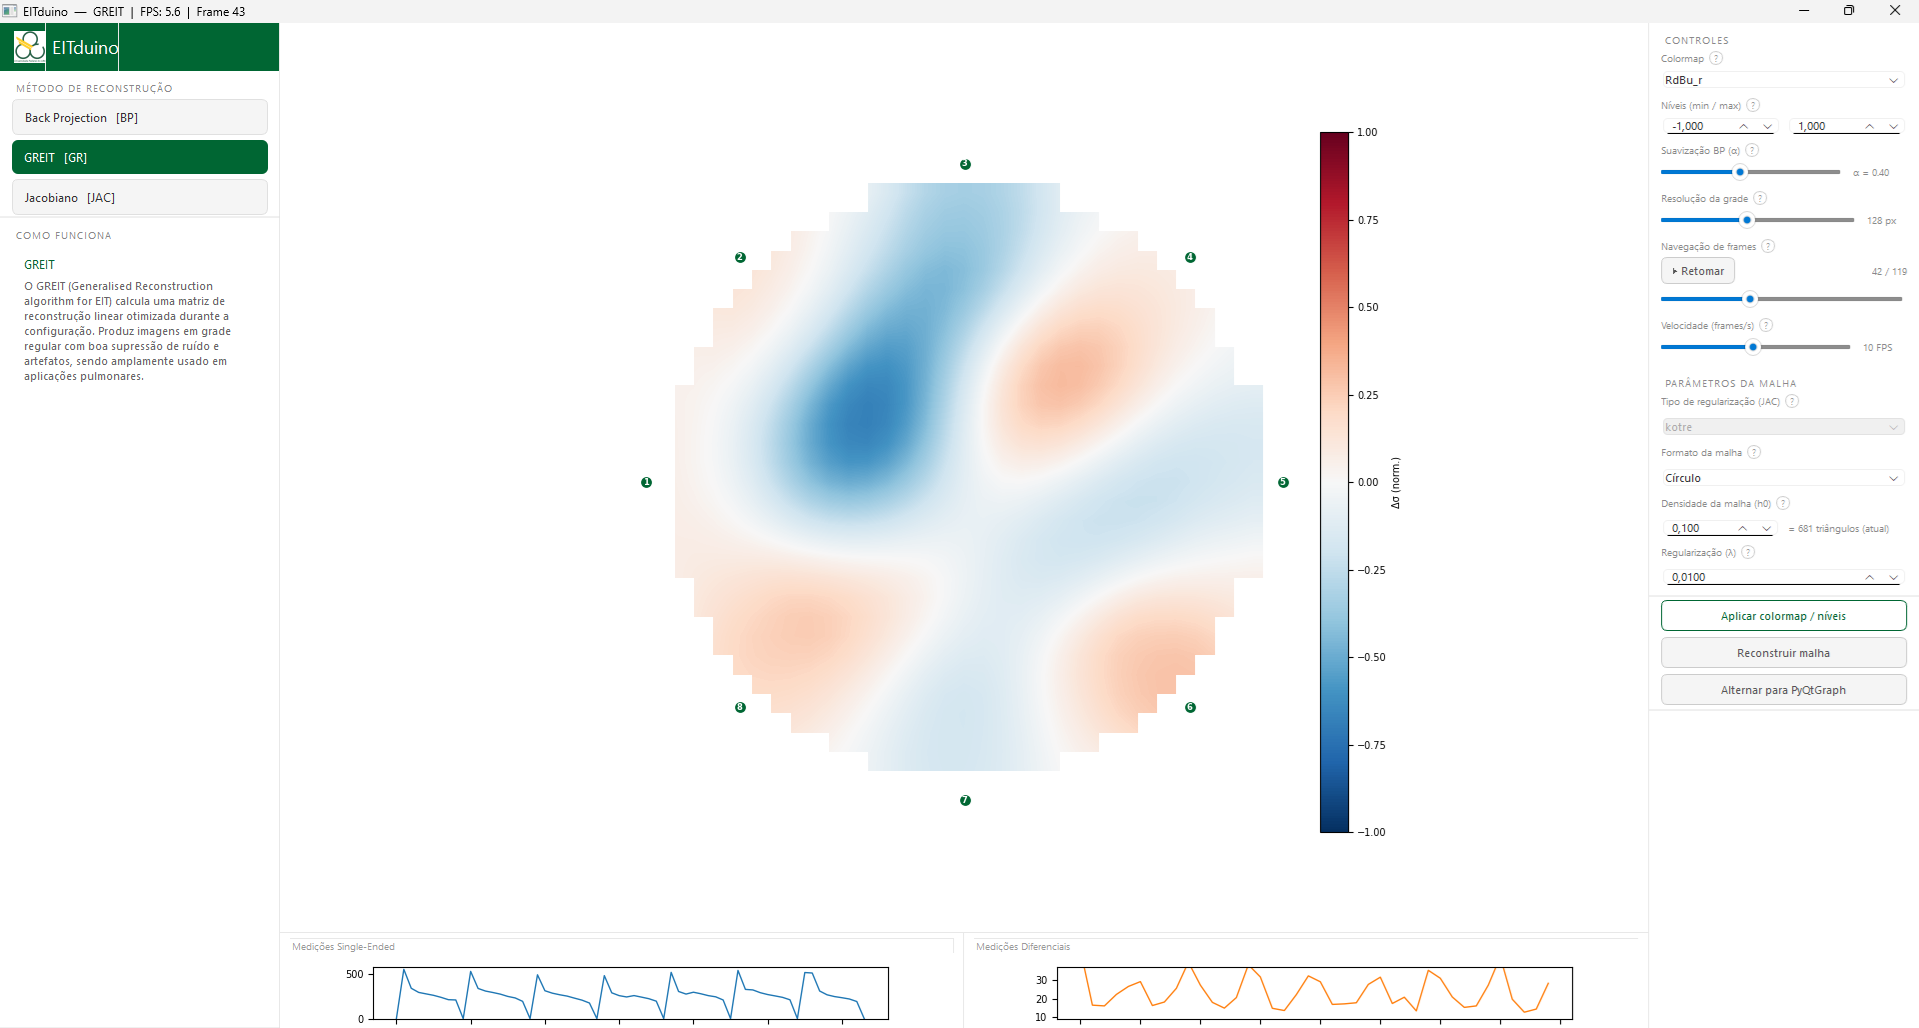
\includegraphics[width=0.85\textwidth]{pictures/GREIT_pyQT_Reg0_01.png}
    \caption{Reconstrução obtida com o método GREIT no \textit{frame} 43, utilizando \(\lambda = 0{,}01\).}
    \label{fig:greit_reg_001}
\end{figure}

\begin{figure}[htbp]
    \centering
    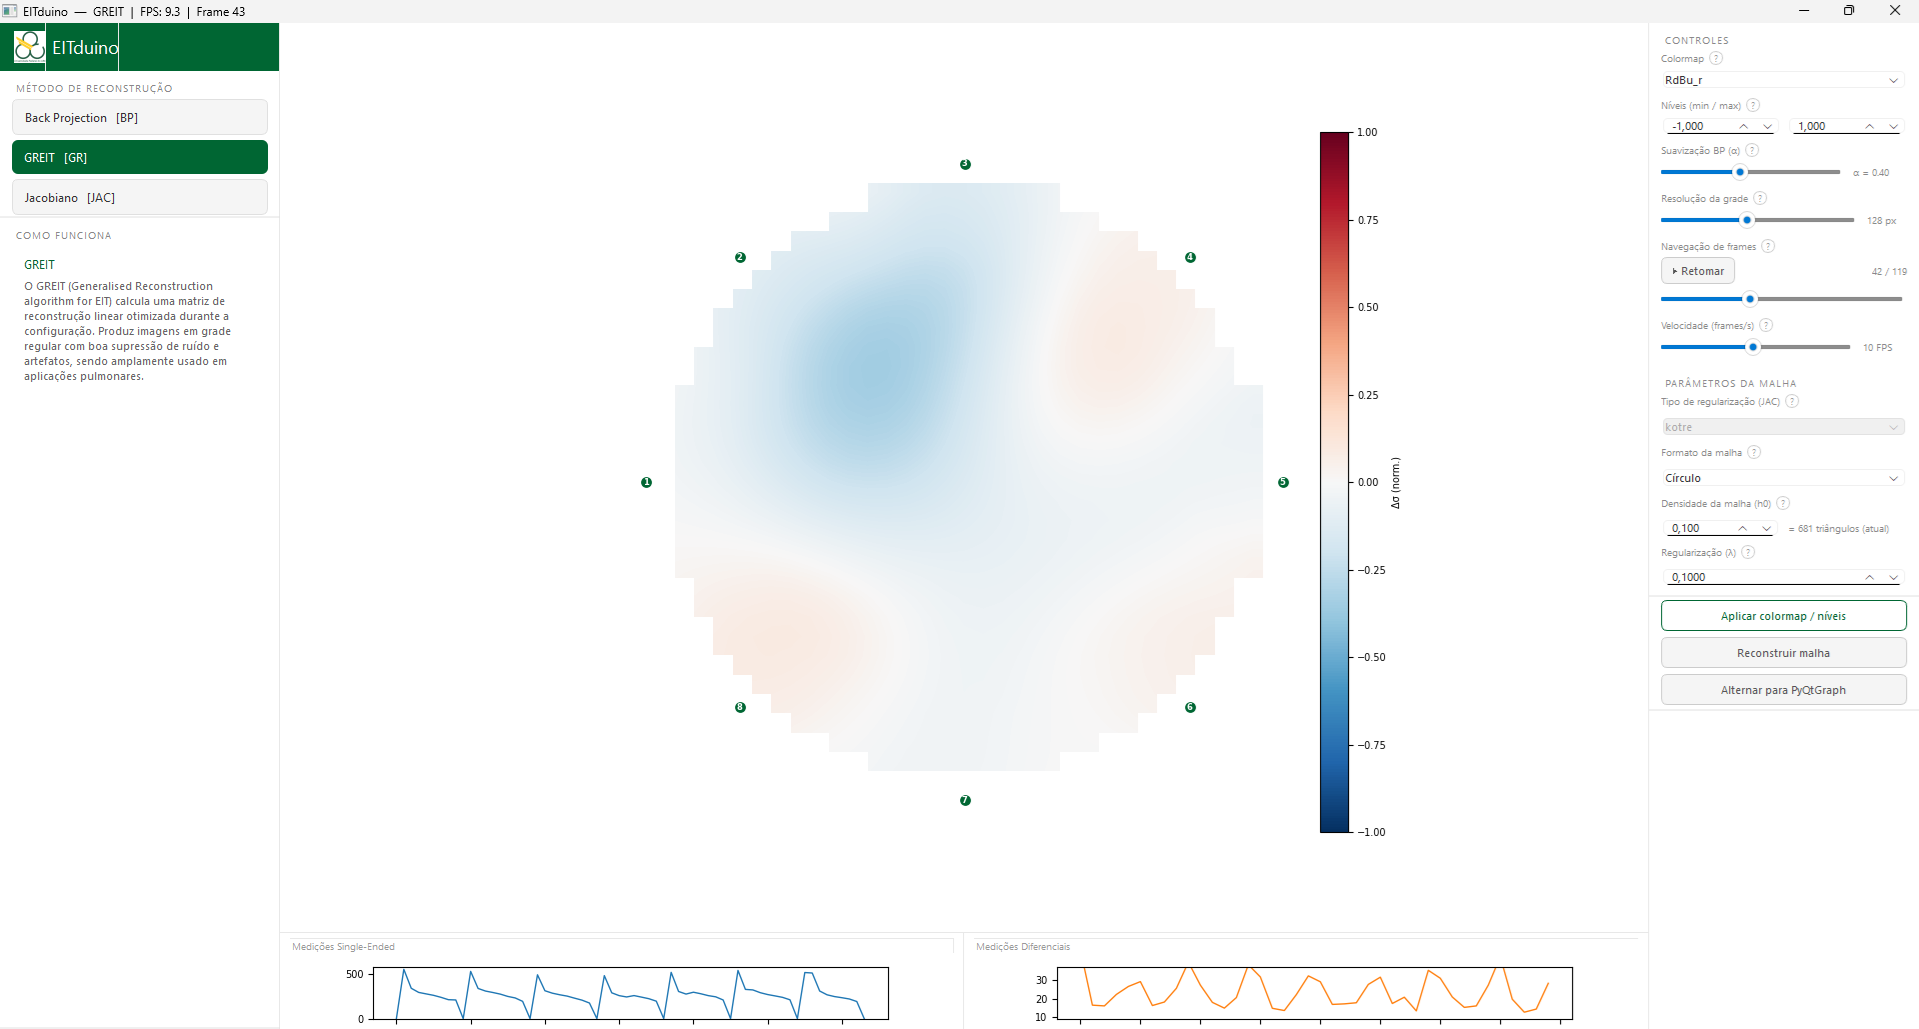
\includegraphics[width=0.85\textwidth]{pictures/GREIT_pyQT_Reg0_1.png}
    \caption{Reconstrução obtida com o método GREIT no \textit{frame} 43, utilizando \(\lambda = 0{,}1\).}
    \label{fig:greit_reg_01}
\end{figure}

\begin{figure}[htbp]
    \centering
    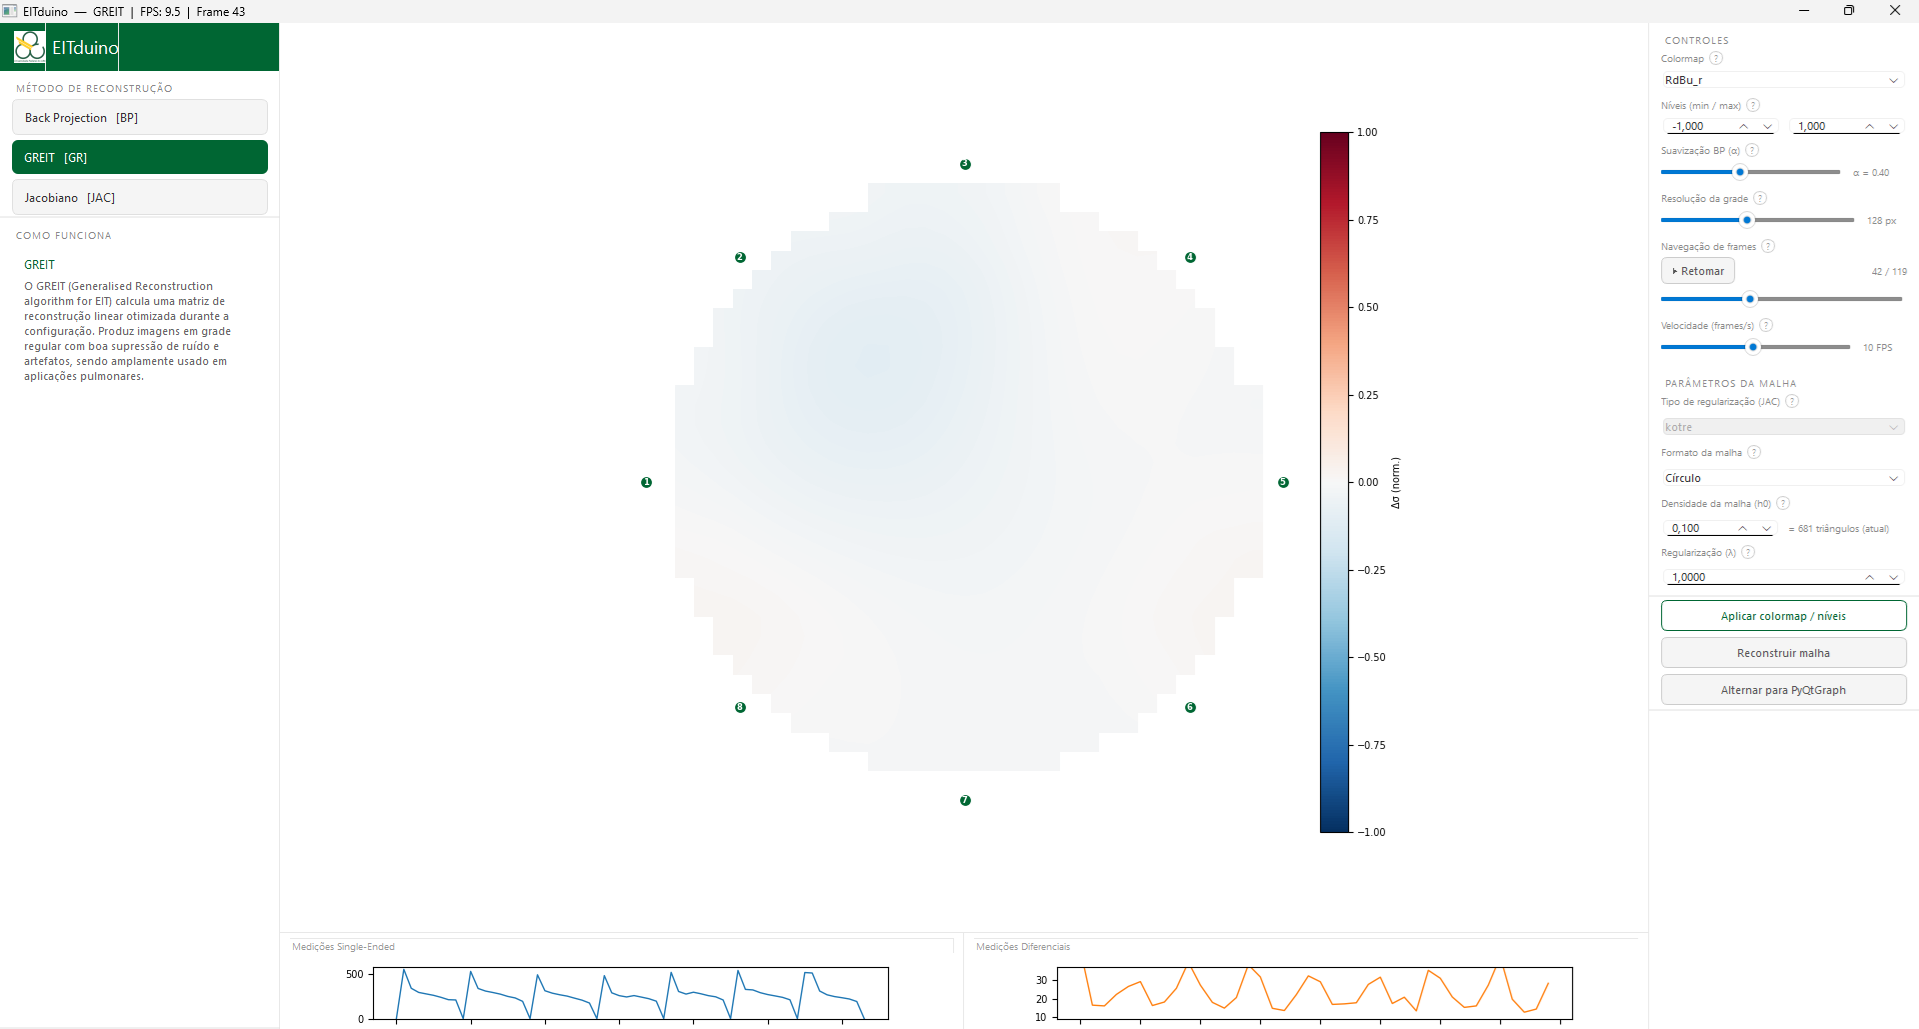
\includegraphics[width=0.85\textwidth]{pictures/GREIT_pyQT_Reg1.png}
    \caption{Reconstrução obtida com o método GREIT no \textit{frame} 43, utilizando \(\lambda = 1{,}0\).}
    \label{fig:greit_reg_1}
\end{figure}

\clearpage

\section{Interface PyQtGraph}
\label{sec:interface_pyqtgraph_resultados}

A interface alternativa desenvolvida com PyQtGraph foi implementada como uma prova de conceito funcional para uma segunda estratégia de visualização das reconstruções. Sua organização foi estruturada em três abas principais: a aba \textit{Solver}, destinada à seleção do método de reconstrução e à exibição de uma descrição resumida do algoritmo ativo; a aba \textit{Controls}, que reúne os parâmetros de visualização e de reconstrução disponíveis nessa implementação; e a aba \textit{Measurements}, voltada à exibição das curvas associadas aos sinais medidos. Em contraste com a interface principal, baseada em uma disposição fixa em painéis, essa versão adota uma organização mais compacta e concentra os controles laterais em abas, preservando os elementos centrais do fluxo de reconstrução. Embora disponha de menos controles do que a interface principal, essa implementação mantém a mesma camada de reconstrução baseada na classe \texttt{EITsolver}. Do ponto de vista arquitetural, a diferença principal está na camada de visualização: a interface em PyQtGraph utiliza \texttt{pg.ImageView} para exibição da imagem reconstruída e \texttt{pg.PlotWidget} para as curvas dos sinais, substituindo o canvas do Matplotlib empregado na interface principal.

\begin{figure}[htbp]
    \centering
    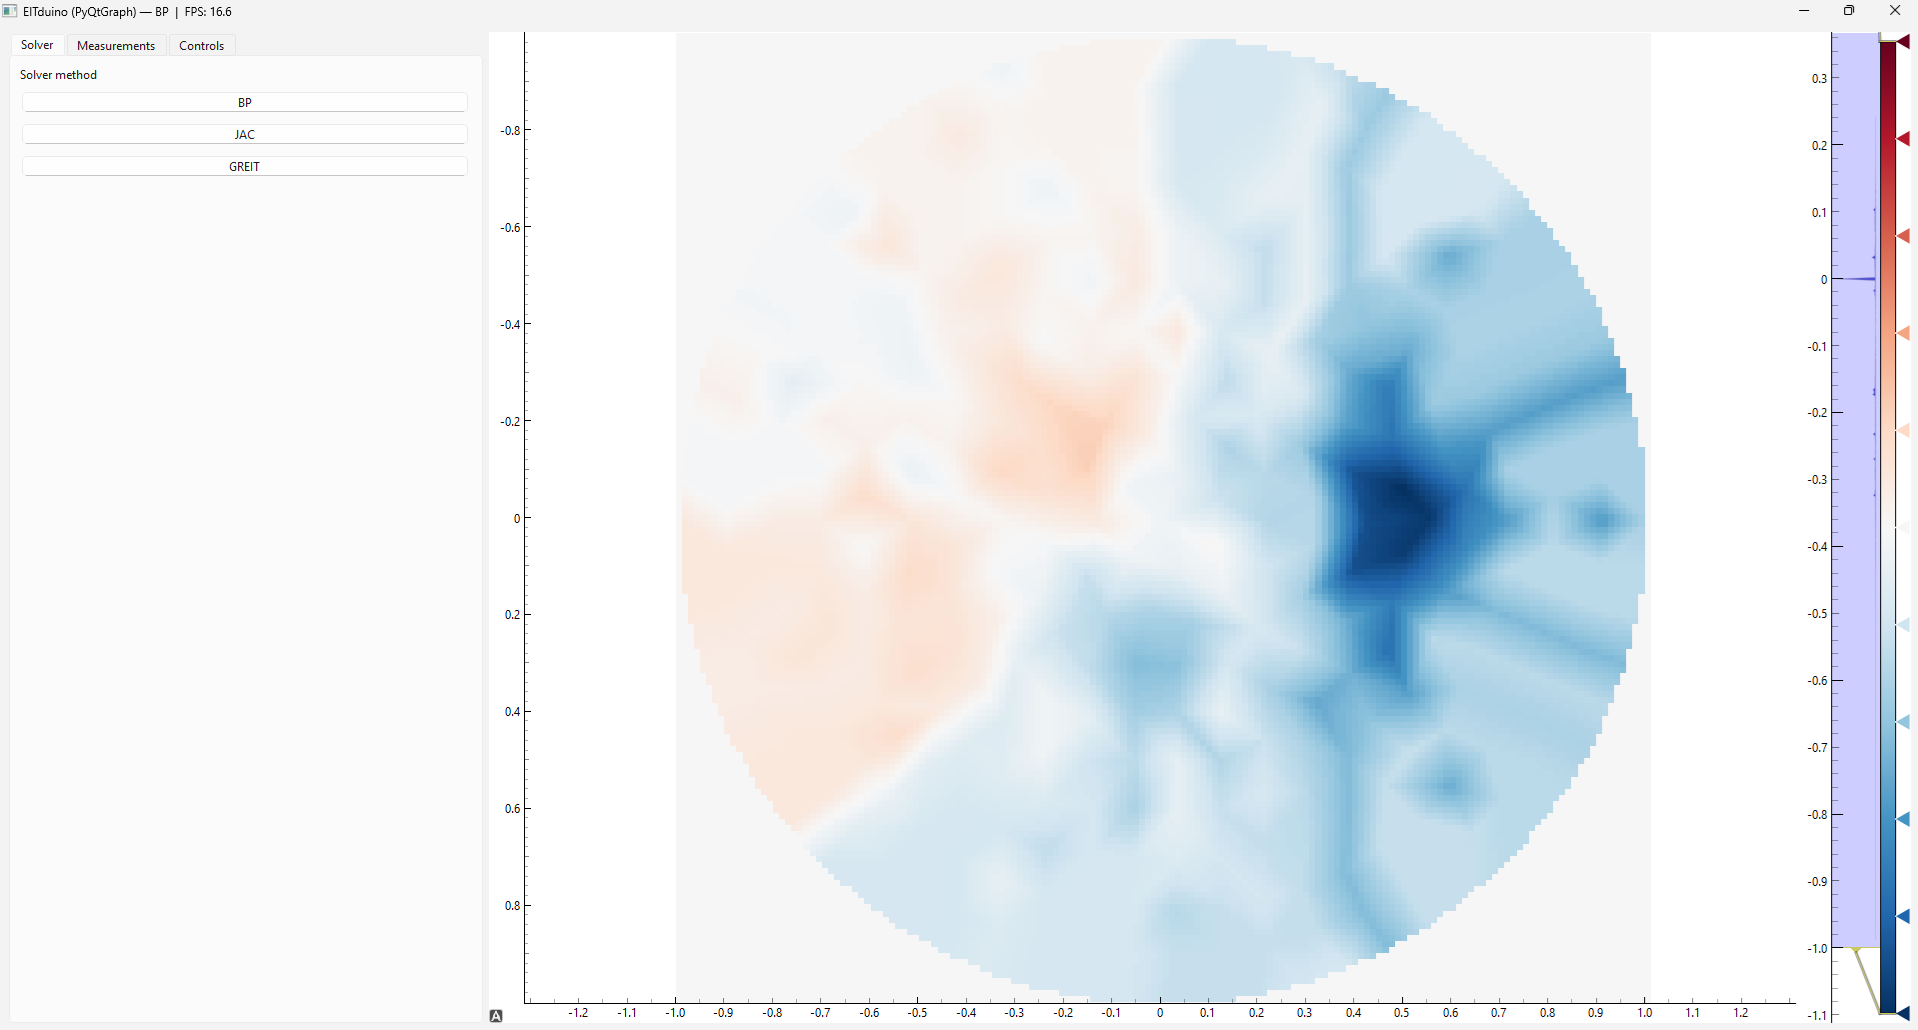
\includegraphics[width=0.85\textwidth]{pictures/BP_PyQtGraph_SolverTab.png}
    \caption{Visão geral da interface alternativa baseada em PyQtGraph, com a aba \textit{Solver} ativa.}
    \label{fig:pyqtgraph_solver_tab}
\end{figure}

\begin{figure}[htbp]
    \centering
    \begin{minipage}{0.48\textwidth}
        \centering
        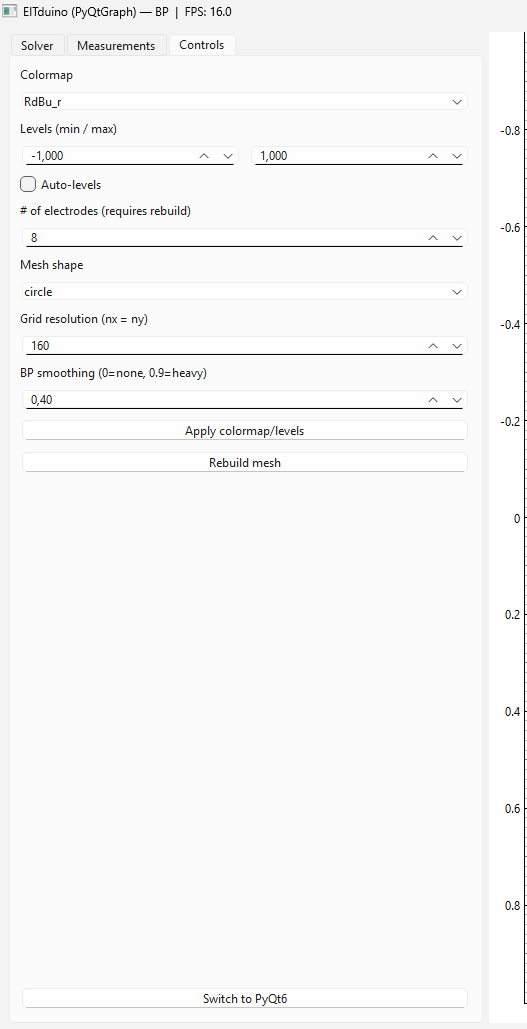
\includegraphics[width=\textwidth]{pictures/BP_PyQtGraph_ControlTab.png}
        \caption*{(a) Aba \textit{Controls}}
    \end{minipage}
    \hfill
    \begin{minipage}{0.48\textwidth}
        \centering
        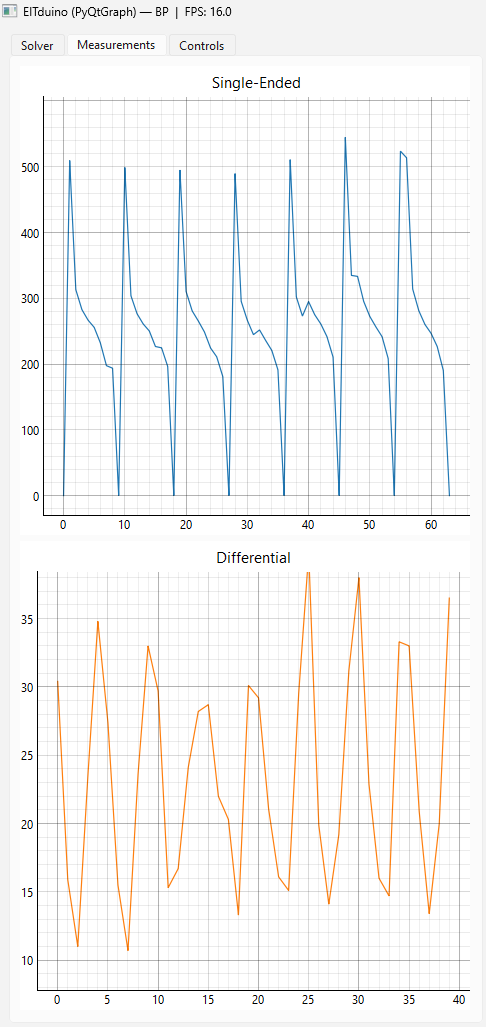
\includegraphics[width=\textwidth]{pictures/BP_PyQtGraph_MeasurementsTab.png}
        \caption*{(b) Aba \textit{Measurements}}
    \end{minipage}
    \caption{Detalhes da interface PyQtGraph com foco nas abas laterais de configuração e visualização dos sinais.}
    \label{fig:pyqtgraph_tabs}
\end{figure}
